\documentclass[12pt]{article}
\usepackage[english]{babel}
\usepackage{url}
\usepackage[utf8]{inputenc}
\usepackage{rotating}
\usepackage{listings}
\usepackage[
backend=biber,
style=numeric,
urldate=long
]{biblatex}
\usepackage{booktabs}
\newcommand{\tabitem}{\makebox[1em][r]{\textbullet~}}
\usepackage{amsmath}
\usepackage{graphicx}
\graphicspath{{images/}}
\usepackage{parskip}
\usepackage{fancyhdr}
\usepackage{vmargin}
\usepackage{float}
\usepackage{chngcntr}
\usepackage [autostyle, english = british]{csquotes}
\MakeOuterQuote{"}
\usepackage[justification=centering]{caption}
\usepackage{subcaption}
\counterwithin{figure}{section}
\counterwithin{table}{section}
\setmarginsrb{3 cm}{2.5 cm}{3 cm}{2.5 cm}{1 cm}{1.5 cm}{1 cm}{1.5 cm}

\usepackage{xcolor}

\colorlet{punct}{red!60!black}
\definecolor{background}{HTML}{EEEEEE}
\definecolor{delim}{RGB}{20,105,176}
\colorlet{numb}{magenta!60!black}

\lstdefinelanguage{json}{
    basicstyle=\normalfont\ttfamily,
    numbers=left,
    numberstyle=\scriptsize,
    stepnumber=1,
    numbersep=8pt,
    showstringspaces=false,
    breaklines=true,
    frame=lines,
    backgroundcolor=\color{background},
    literate=
     *{0}{{{\color{numb}0}}}{1}
      {1}{{{\color{numb}1}}}{1}
      {2}{{{\color{numb}2}}}{1}
      {3}{{{\color{numb}3}}}{1}
      {4}{{{\color{numb}4}}}{1}
      {5}{{{\color{numb}5}}}{1}
      {6}{{{\color{numb}6}}}{1}
      {7}{{{\color{numb}7}}}{1}
      {8}{{{\color{numb}8}}}{1}
      {9}{{{\color{numb}9}}}{1}
      {:}{{{\color{punct}{:}}}}{1}
      {,}{{{\color{punct}{,}}}}{1}
      {\{}{{{\color{delim}{\{}}}}{1}
      {\}}{{{\color{delim}{\}}}}}{1}
      {[}{{{\color{delim}{[}}}}{1}
      {]}{{{\color{delim}{]}}}}{1},
}

\title{News Aggregator and Summariser}								% Title
\author{Kunal M L Wagle}								% Author
\date{\today}											% Date


\addbibresource{sample.bib}

\DefineBibliographyStrings{english}{%
urlseen = {Retrieved},
}

\makeatletter
\let\thetitle\@title
\let\theauthor\@author
\let\thedate\@date
\makeatother

\usepackage{imakeidx}
\indexsetup{othercode=\small}
\makeindex[program=makeindex,columns=2,intoc=true,options={-s mystyle.ist}]

\pagestyle{fancy}
\fancyhf{}
\rhead{\theauthor}
\lhead{\thetitle}
\cfoot{\thepage}

\begin{document}

%%%%%%%%%%%%%%%%%%%%%%%%%%%%%%%%%%%%%%%%%%%%%%%%%%%%%%%%%%%%%%%%%%%%%%%%%%%%%%%%%%%%%%%%%

\begin{titlepage}
	\centering
    \vspace*{0.5 cm}
    
\includegraphics[scale = 0.05]{Imperial_College_London_crest.png}\\[1.0 cm]	% University Logo
    \textsc{\LARGE Imperial College London}\\[2.0 cm]	% University Name
	\textsc{\Large C401}\\[0.5 cm]				% Course Code
	\textsc{\large MEng Computing Interim Report}\\[0.5 cm]				% Course Name
	\rule{\linewidth}{0.2 mm} \\[0.4 cm]
	{ \huge \bfseries \thetitle}\\
	\rule{\linewidth}{0.2 mm} \\[1.5 cm]
	
	\begin{minipage}{0.4\textwidth}
		\begin{flushleft} \large
			\emph{Author:}\\
			\theauthor
			\end{flushleft}
			\end{minipage}~
			\begin{minipage}{0.4\textwidth}
			\begin{flushright} \large
			\emph{Supervisor:} \\
			Anandha Gopalan									% Your Student Number
		\end{flushright}
	\end{minipage}\\[2 cm]
	
	{\large \thedate}\\[2 cm]
 
	\vfill
	
\end{titlepage}

%%%%%%%%%%%%%%%%%%%%%%%%%%%%%%%%%%%%%%%%%%%%%%%%%%%%%%%%%%%%%%%%%%%%%%%%%%%%%%%%%%%%%%%%%

\tableofcontents
\pagebreak
\listoffigures
\listoftables
\pagebreak

%%%%%%%%%%%%%%%%%%%%%%%%%%%%%%%%%%%%%%%%%%%%%%%%%%%%%%%%%%%%%%%%%%%%%%%%%%%%%%%%%%%%%%%%%

\section{Introduction}

In a fast moving world it's more important now than ever to stay on top of the news. However, people are often faced with their own questions when they're searching for news: Where should I get it from? How many sources should I use to ascertain the facts about a piece of news? Can I trust this source and what it is saying?

Coupled with these questions is a study by the Statistic Brain Research Institute\cite{statisticBrain}\index{Statistic Brain Research Institute} that suggests that the average attention span\index{Attention span} of a person has dropped significantly over the last five years\cite{attentionSpan}. There is arguably more news and more sources to read news from, but even less time in which to read it all.

There are potentially hundreds of different sources\index{Source} for articles on a single piece of news. For example, if I were to search Google News\cite{googleNews}\index{Google!News} (on the 22nd December 2016) for "Uber"\index{Uber} I would be greeted with articles about the fact that Uber\cite{uber} have been forced to withdraw driverless cars from the roads of San Francisco\index{San Francisco}. Upon further examination, it becomes clear that Google News has a similar story from as many as 50-60 sources. But which one should we read from?

My project aims to resolve some of these issues, by creating a new platform that aggregates news from a variety of different news sources, merges articles about the same specific piece of news, and summarises them. This would thus provide news for readers in short pieces, allowing a user to cover more of the news than ever before.

The first aim of the project is to create a news aggregator. One of the key differentials between this and the current news aggregators on the market (such as Flipboard\cite{flipboard}\index{Flipboard}) would be that with my project, users will be able to search for news related to much more specific topics than currently offered. 

One of the main aims of the project would be to identify "duplicate"\index{Duplicate} articles (articles that are about the same story) and merge them into one article for the user to read. However, this could of course raise the issue that articles suddenly become too long for a user to read. This is addressed below. 

With a key issue for users now being the time factor, an aim of the project would be to reduce the time needed for a user to surmise the key issues and facts of a news story. To do this, there are two key issues - the sources\index{Source} for the articles, and the length of the articles. 

An issue with some articles is the length. In July 2016 a study was conducted by the Statistic Brain Research Institute\cite{statisticBrain}\index{Statistic Brain Research Institute} that said that the average attention span\index{Attention span} of a person is now as low as 8.25 seconds\cite{attentionSpan}. In addition to this, the Institute's findings also said that the average person only reads 28\% of a webpage of average length (593 words). Another key finding was that users spend only 4.4 seconds to cover each additional 100 words on a webpage. 

With this in mind, it becomes clear that a key problem with articles is that they're too long for the average user. If a key point is not mentioned in the article until near the end, it's more than possible that the user could miss it entirely. As a result, a key aim of this project must be to try and counteract this issue.

The best way to do this is to find a way to summarise the article so that the users can see the key facts at a glance. The project would aim to automatically summarise the merged articles found by the duplication\index{Duplication} algorithm. This would be a key differential between my project and news aggregators\index{News Aggregator} on the market.

On a personal level, something I've noticed in the past about alternative news aggregators\index{News Aggregator} available is that it's not easy in many cases to tailor the sources that you get your news from. To take an extreme example, someone who normally reads \emph{The Guardian}\cite{guardian}\index{Guardian, The} is unlikely to want to get their news from \emph{Fox News}\cite{foxNews}\index{Fox News}, as they are on opposite ends of the political spectrum. 

As a result, a secondary aim of the project would be to allow a user to customise the sources that they receive their news from. One potential way to do this would be to present the user with a list of news sources\index{Source} that the project will source news from, and allow them to remove selections as necessary. The article could then be summarised so that only news from those sources is present in the final version presented to the users.

However, this could have its own pitfalls, despite the obvious benefits. 

One of the more interesting findings in the 2016 Digital News Report\index{Digital News Report}\cite{digitalNewsReport} (conducted by the Reuters Institute for the Study of Journalism\cite{reutersInstitute}\index{Reuters Institute for the Study of Journalism}) was that some were concerned about the potential impact of personalising their news feeds. They felt that it could lead to both "missing information" and "missing challenging viewpoints". A secondary aim of the project would be to find a way to rectify this misgiving. This could potentially be done in different ways, from providing summarisation of articles from alternate sources of the article, or by simply posting a link to articles about the same topic from sources considered to be on the opposite end of the political spectrum. 

\pagebreak

\section{Market Research}

\subsection{News Reading Habits}

\subsubsection{Digital News Report 2016}

\label{DigitalNewsReport}

Conducted by the Reuters Institute for the Study of Journalism\cite{reutersInstitute}\index{Reuters Institute for the Study of Journalism} in Oxford University\cite{oxford}\index{University of Oxford}, the Digital News Report\index{Digital News Report}\cite{digitalNewsReport} is an annual study that serves to investigate how people access and find out about news in various countries across the globe, including the United Kingdom\index{United Kingdom}.

The study attempts to cover, amongst other things how people get the news, how they use social media\index{Social Media}, what types of news they trust, and both the reasons to use and concerns about news aggregators. Findings of the report relevant to my concept are listed below:

\textbf{Reasons to use News Aggregators\index{News Aggregator!Reasons for use}}

\begin{figure}[h]
  \centering
    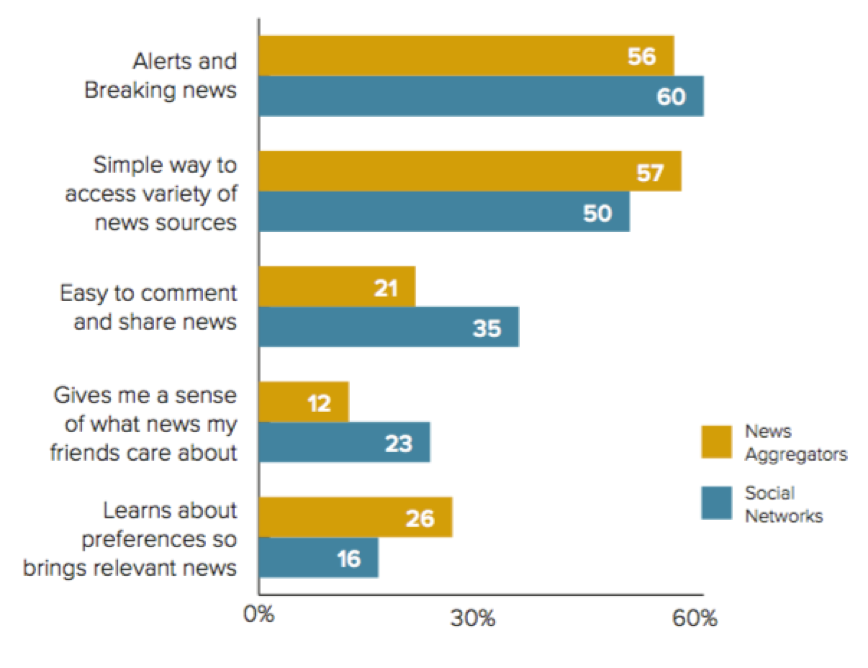
\includegraphics[scale=0.6]{WhySocialAggregatedNews.png}
   \caption[Why people use News Aggregators]{A graph showing why people use News Aggregators and Social Networks as news sources}
   \label{WhySocialAggregatedNews}
\end{figure}

As shown in the graph in Figure \ref{WhySocialAggregatedNews} the key to the popularity of a News Aggregator is that it's simplicity and speed. It's important to bring news as soon as it happens, and it needs to provide access to a variety of different news sources. Of lesser importance is the social aspect - the need to comment and share the news, although the fact that 26\% of people want their preferences to influence the news that they're interested in should not be discounted.

\textbf{Concerns about Personalised News\index{News ! Personalised}}

\begin{figure}[h]
  \centering
    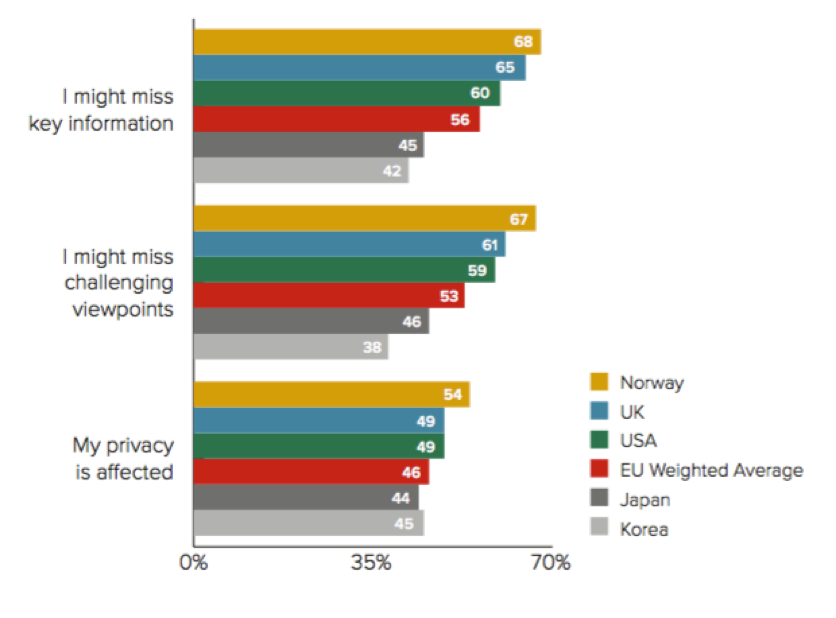
\includegraphics[scale=0.6]{PersonalisedNewsConcerns.png}
   \caption[Concerns with personalisation of News Feeds]{A graph showing the main three concerns that people have with Personalised News Feeds determining what they read.}
   \label{PersonalisedNewsConcerns}
\end{figure}

Key concerns, especially in the United Kingdom\index{United Kingdom}, with Personalised News\index{News ! Personalised} is that information might be incomplete. It is not difficult to see why this may be a concern - if you limit your news to a subset of the sources that might be available then it's possible to miss parts of the story - the parts that challenge aspects of the articles you're reading. It's therefore important that the project reflects this concern, which is why it is listed as a secondary aim (See section \ref{ChallengingViewpoints}). \\

\textbf{What should determine what someone reads next}

\begin{figure}[h]
  \centering
    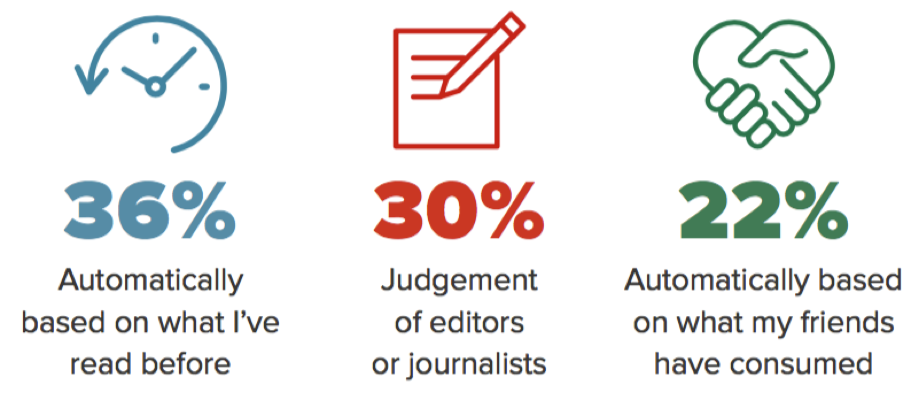
\includegraphics[scale=0.6]{HowPeopleTrustNews.png}
   \caption[What is a good way to get to the news?]{Key statistics in response to the question: Is this a good way to get the news?}
   \label{HowPeopleTrustNews}
\end{figure}

Least popular are algorithms that present news based on what people's friends have been reading. In general, according to the Reuters Institute\cite{reutersInstitute}\index{Reuters Institute for the Study of Journalism}, "People think *they* are the best judge of what's important to them." More interesting, is that people are now less inclined to allow journalists or editors to push articles to the top of reading lists than having an algorithm suggest similar stories to what they've just consumed. This could perhaps indicate that they aren't as trusting in journalists and editors as before - something that the Reuters Institute\index{Reuters Institute for the Study of Journalism} touches upon in an essay near the end of the report. \\

\textbf{Conclusions}

The Reuters Institute for the Study of Journalism\index{Reuters Institute for the Study of Journalism} is a trusted and respected organisation, and this study has been supported by institutions varying from media outlets such as the BBC\cite{bbc}\index{BBC}, news search engines such as Google\index{Google}\index{Google!Search Engine}, and other Universities, such as University of Canberra\cite{canberra}\index{University of Canberra}. Importantly, it's also supported by regulators, including Ofcom\cite{ofcom}\index{Ofcom}, which is the regulator in the United Kingdom\index{United Kingdom}. 

The survey was conducted on their behalf by YouGov\cite{yougov}\index{YouGov}, which is a highly respected polling company in the United Kingdom\index{United Kingdom}, and it surveyed more than 50,000 people, including over 2000 in the United Kingdom. In addition, the report is coupled with numerous essays on various key points that arose from the study. The writers of these essays varied from the Director of Research at the Reuters Institute\index{Reuters Institute for the Study of Journalism} to the Chief Executive Officer of The New York Times\cite{newYorkTimes}\index{New York Times}.

As a result of this, I deemed the Digital News Report 2016\index{Digital News Report}\cite{digitalNewsReport} to be a very reliable source of information with regards to how people read the news, and their preferences in the field. 

\subsubsection{Potential User Survey\index{User!Survey}}

\label{survey}

Following this initial research I decided to conduct a survey of potential users to delve into more specific aspects of News Reading Habits. I was more focused on the number of sources people use to ascertain the facts about a piece of news. I also asked questions regarding the summarisation\index{Summarisation} of news and news digests.

I was interested in the questions about summarisation and digests after reading some data from a study conducted by the Statistic Brain Research Institute\cite{statisticBrain}\index{Statistic Brain Research Institute}. Statistic Brain conducted a study in July 2016 that suggested that the average attention span of a human is now only 8.25 seconds\cite{attentionSpan}. They coupled the presentation of this data with statistics about people browsing the internet taken from the paper \emph{Not Quite the Average:
An Empirical Study of Web Use}\index{Not Quite the Average: An Empirical Study of Web Use}\cite{empiricalStudyofWebUse}. The statistics suggest that the average user only reads 28\% of the words on the average webpage, and that for each additional 100 words beyond that, the user would only spend an additional 4.4 seconds on the page.

Admittedly, the paper was written in 2008, and so might not reflect average web browsing activity, but it raised a question worth answering in my opinion. Do users actually read full articles on the news, and if not, would summarising articles help make sure they didn't miss out on key points, thus counteracting an issue discovered in the Digital News Report 2016\index{Digital News Report}\cite{digitalNewsReport} (Section \ref{DigitalNewsReport})? 

The survey was presented on Google Forms\cite{googleForms}\index{Google!Forms} and was answered by 96 respondents. Further findings are shown below:

\begin{enumerate}

\item \textbf{How often do you read the news?}

\begin{figure}[ht!]
  \centering
    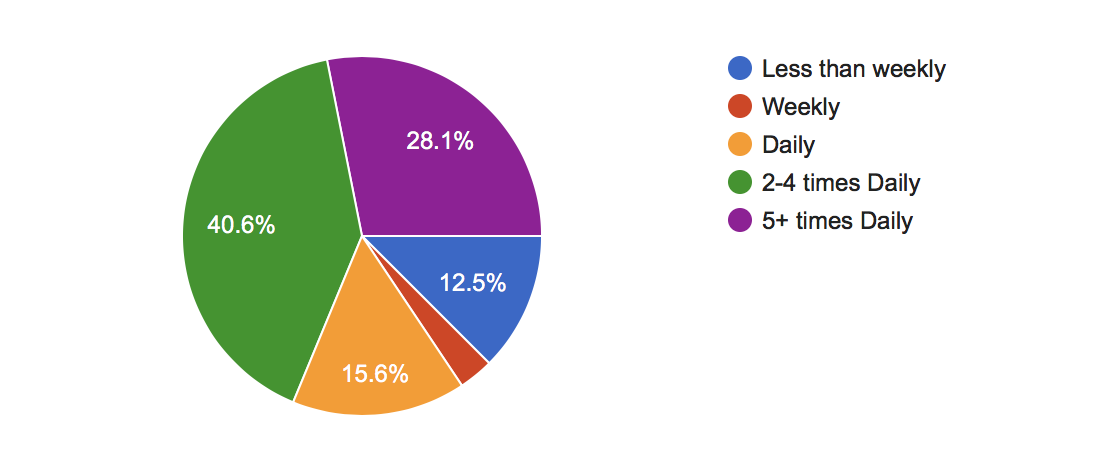
\includegraphics[scale=0.7]{01HowOftenDoYouReadTheNews}
   \caption[Survey Graph surrounding how often news is read]{A pie chart showing how often people read the news.}
   \label{SurveyHowOftenDoYouReadTheNews}
\end{figure}

The first question (Figure \ref{SurveyHowOftenDoYouReadTheNews}) on the survey was designed to ascertain how often people read the news. Overall, well over 80\% of respondents said that they read the news at least daily, and nearly 60\% more than once per day. \\

\item \textbf{How many sources do you read?}

\begin{figure}[ht!]
  \centering
    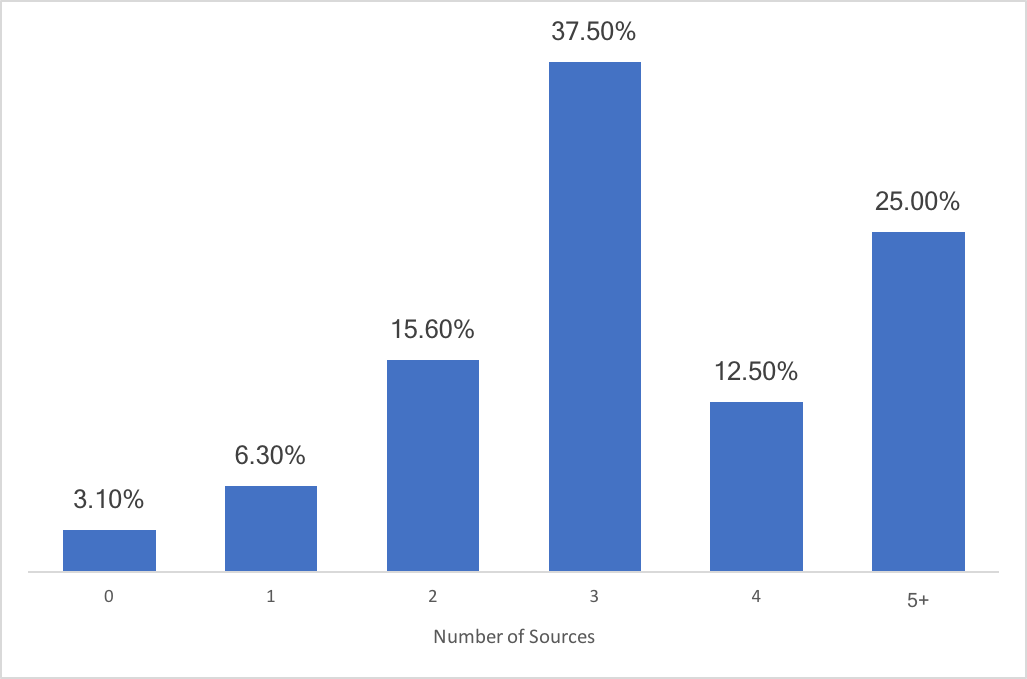
\includegraphics[scale=0.7]{02HowManySourcesDoYouRead}
   \caption[Survey Graph asking how many sources are used]{A bar graph showing how many sources people normally use for a source of news.}
   \label{SurveySources}
\end{figure}

Next I asked about how many sources a user read. It was quite rare for someone to use only one source for a piece of news. In fact, over 90\% said that they used two or more sources, with three and five sources being the most prominent selections. \\

\item \textbf{Are these the same sources every time?}

\begin{figure}[ht!]
  \centering
    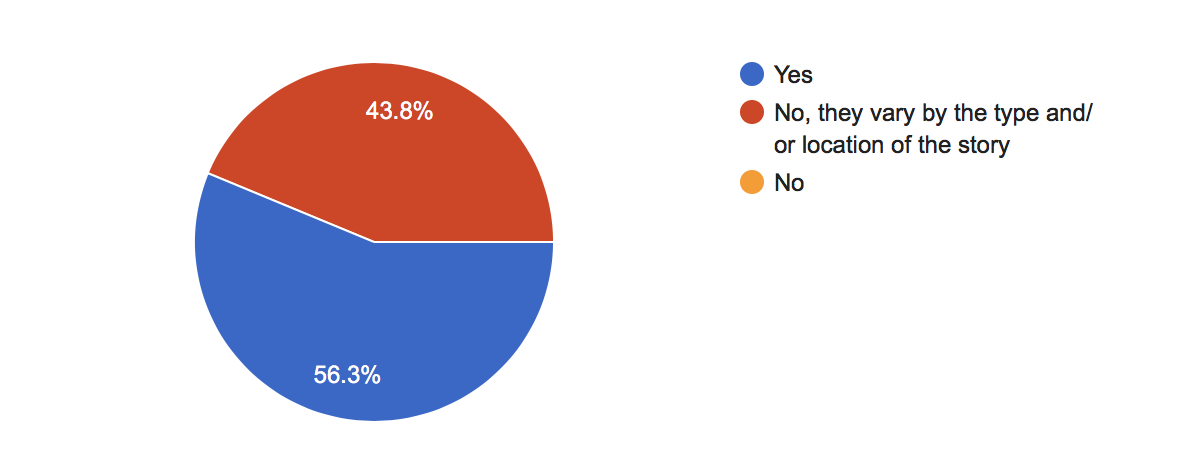
\includegraphics[scale=0.7]{03AreTheseTheSameSourcesEverytime}
   \caption[Survey Graph about consistency of sources]{A pie chart showing whether people use the same sources every time.}
   \label{SurveySourceConsistency}
\end{figure}

The respondents were a lot more split on the question of consistency of sources, although more than half said that they used the same sources every time, with 43.8\% saying that they vary their sources based on the type and/or location of the news story. \\

\item \textbf{How much of an article do you normally read?}

\begin{figure}[ht!]
  \centering
    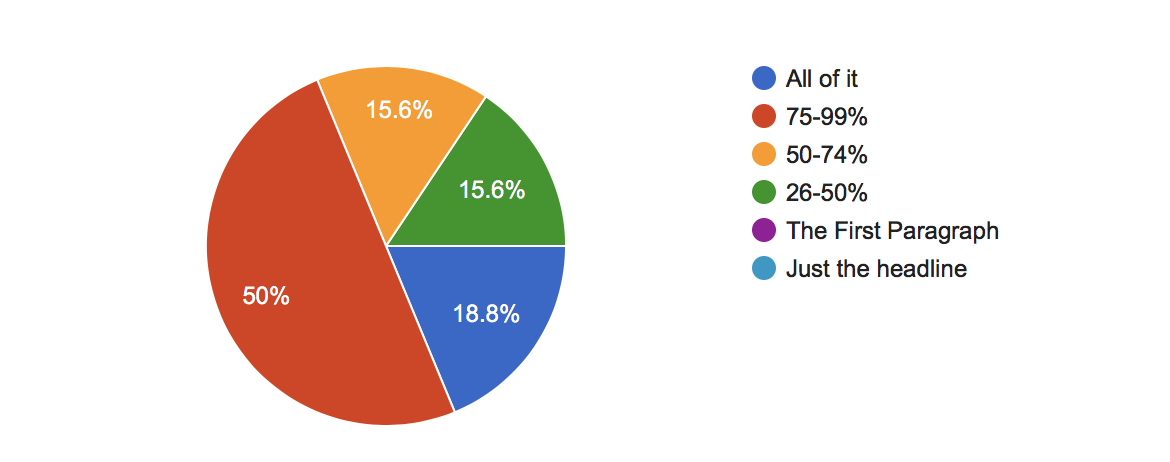
\includegraphics[scale=0.7]{05HowMuchOfAnArticleDoYouRead.png}
   \caption[Survey Graph regarding how much of an article is read]{A pie chart showing how much of articles people normally read.}
   \label{SurveyArticleLength}
\end{figure}

I further expanded upon the initial reading I had done about attention spans by asking potential users how much of articles they normally read. Only 18.8\% of respondents said that they read the entirety of articles (Figure \ref{SurveyArticleLength}), and as much as 15.6\% confess that they read less than 50\% of an article on average. It's plausible that the users could be missing key facts through not reading the entire article. On reflection, I could have also asked if this was a concern to those users. \\

\item \textbf{If an article was presented as a shorter summary, would you read more/all of it?}

\begin{figure}[ht!]
  \centering
    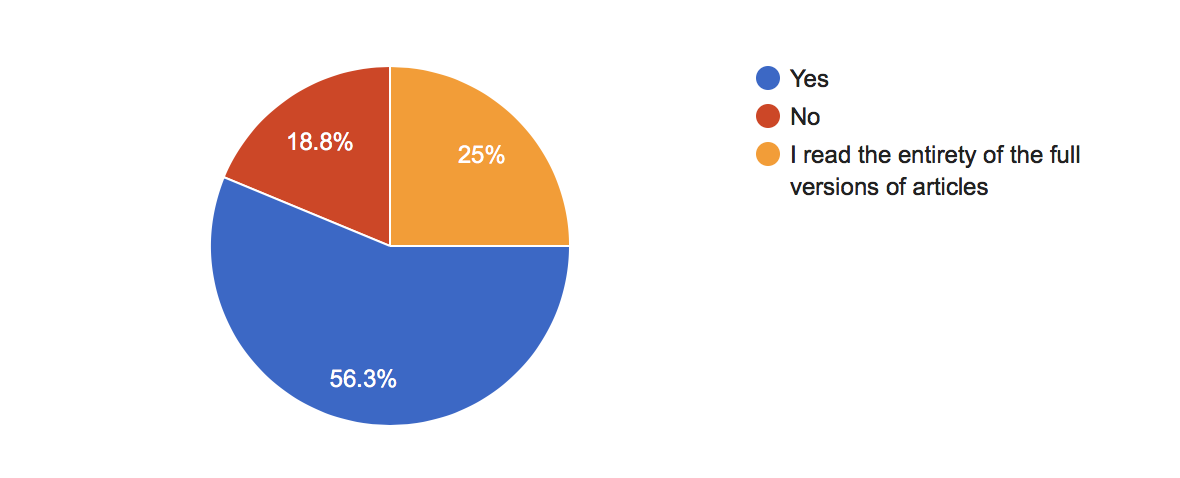
\includegraphics[scale=0.7]{06WouldYouReadAShorterSummary.png}
   \caption[Survey Graph regarding summarisations of articles]{A pie chart showing what percentage of people would read a shorter summary of an article.}
   \label{SurveyArticleLength}
\end{figure}

Another question asked was whether reading a shorter summary would result in users reading more or all of the article. Encouragingly, more than half (56.3\%) of respondents said that they would read a shorter summary. \\

\item \textbf{Would you read a summary of different articles on the same topic combined?}

\begin{figure}[ht!]
  \centering
    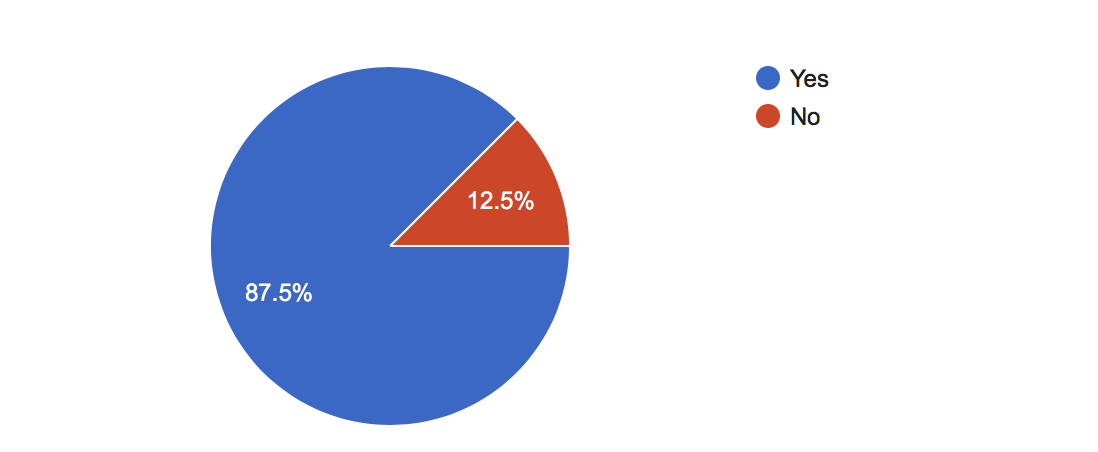
\includegraphics[scale=0.7]{07WouldYouReadASummaryOfArticlesCombined}
   \caption[Survey Graph about combining articles]{A pie chart showing whether people would read a summary of different articles on the same topic combined.}
   \label{SurveySummarisedArticles}
\end{figure}

With this question (Figure \ref{SurveySummarisedArticles}) I aimed to obtain an idea from potential users as to whether combining articles about the same topic from different sources and then summarising it would be considered useful. The question got a resounding response, with as much as 87.5\% saying that they would read a summary like this.  \\

\item \textbf{Would you use a News Aggregator that summarised articles?}

\begin{figure}[ht!]
  \centering
    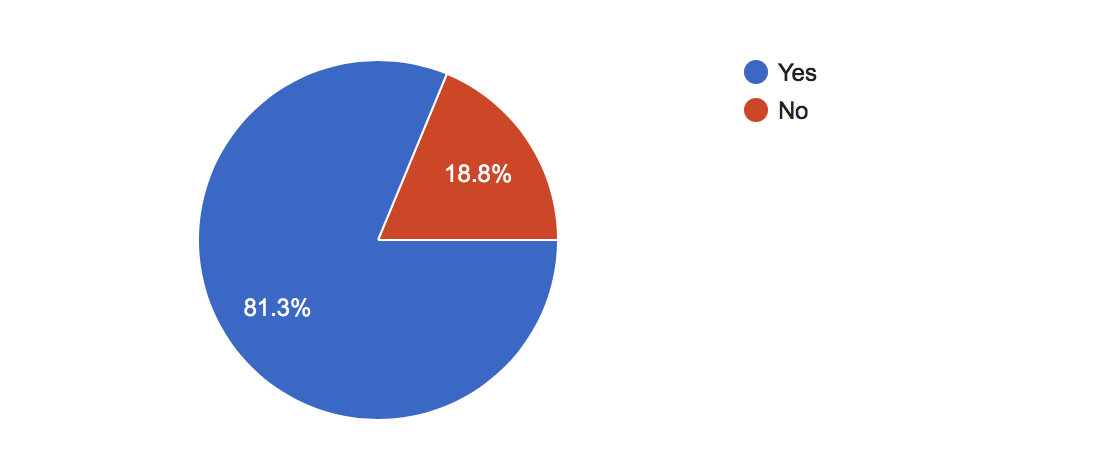
\includegraphics[scale=0.7]{08WouldYouUseANewsAggregatorThatSummarised}
   \caption[Survey Graph concerning News Aggregators and summarisation]{A pie chart showing answers to the question: "Would you use a News Aggregator\index{News Aggregator} that summarised articles"}
  \label{NewsAggregatorThatSummarised}
\end{figure}

Consolidating the findings of the previous question was the fact that 81.3\% said they would use a News Aggregator\index{News Aggregator} that summarised\index{Summarised} articles (Figure \ref{NewsAggregatorThatSummarised}). Amongst those who said they wouldn't, there were comments along the lines of "I'm not great with technology" given as explanation. An interesting comment however, said that "nuance could be lost in the summarisation". This is a valid point, and so a key point of the evaluation\index{Evaluation} process will have to be focused on the summarisation of articles itself, to ensure it's not losing important information at any stage.\\

\item \textbf{How often do you search for news on a specific topic?}

\begin{figure}[ht!]
  \centering
    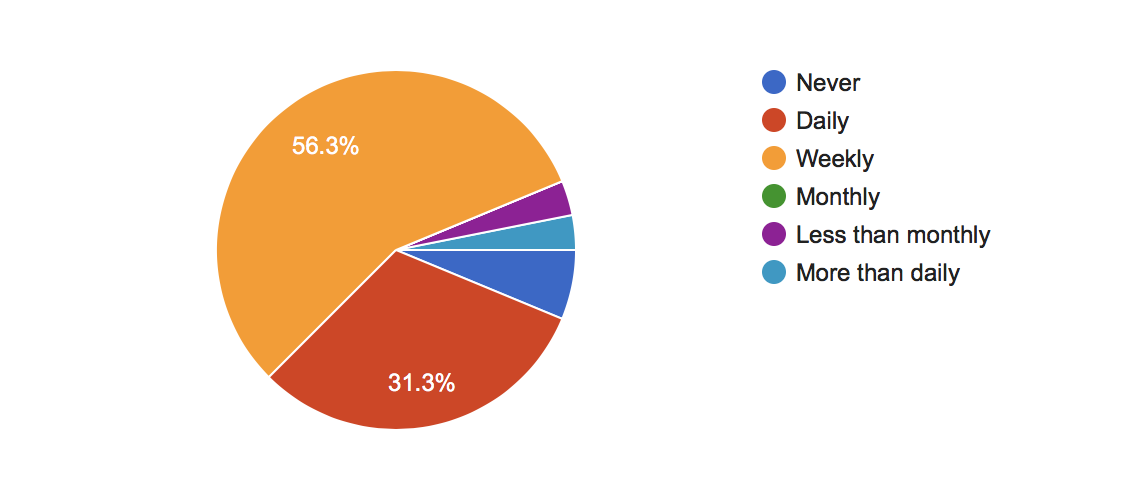
\includegraphics[scale=0.7]{10HowOftenDoYouSearchForASpecificTopic}
   \caption[Survey Graph regarding searching for topics in the news]{A pie chart showing how frequently people search for news on a specific topic.}
   \label{SurveySearchingForTopics}
\end{figure}

For the questions in Figure \ref{SurveySearchingForTopics} I tried to get an idea of how much people search for news on a specific subject of interest to them. In general, this came out to be less frequent then reading the news itself, with just over half the respondents saying that they search for a specific topic weekly. However, a healthy proportion (31.3\%) search daily for specific topics, and some search even more often than this.\\

\item \textbf{Should the news aggregator have the ability to search for a specific topic?}

\begin{figure}[ht!]
  \centering
    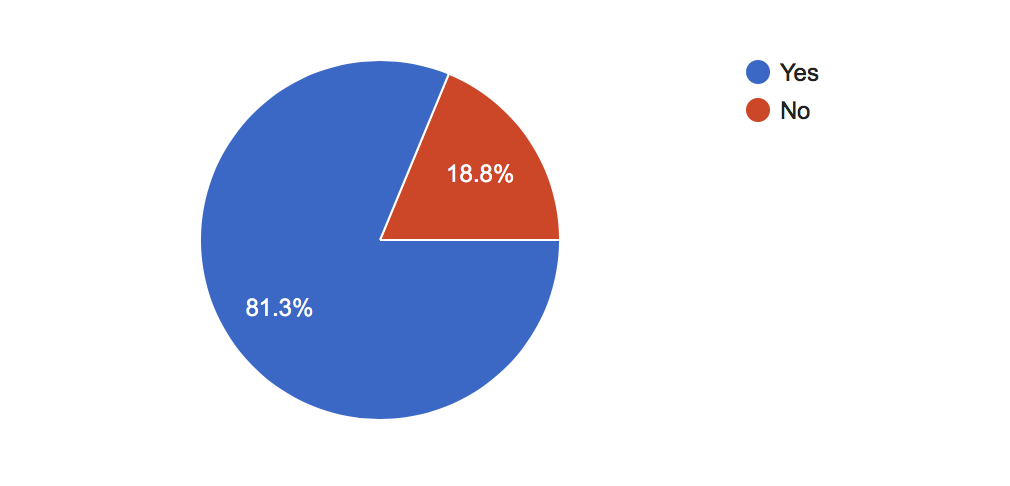
\includegraphics[scale=0.7]{11ShouldNewsAggregatorProvideSearchingForSpecificTopic.png}
   \caption[Survey Graph regarding news aggregators and searching]{The answers to a question asking if the News Aggregator should have the ability to search for a specific topic.}
\end{figure}

As much as 81.3\% of respondents agreed that the News Aggregator\index{News Aggregator} should have a function to search for specific topics. \\

\item \textbf{Do you like services such as news digests that prepare lists of articles each day that apply to a topic you may be interested in?}

\begin{figure}[ht!]
  \centering
    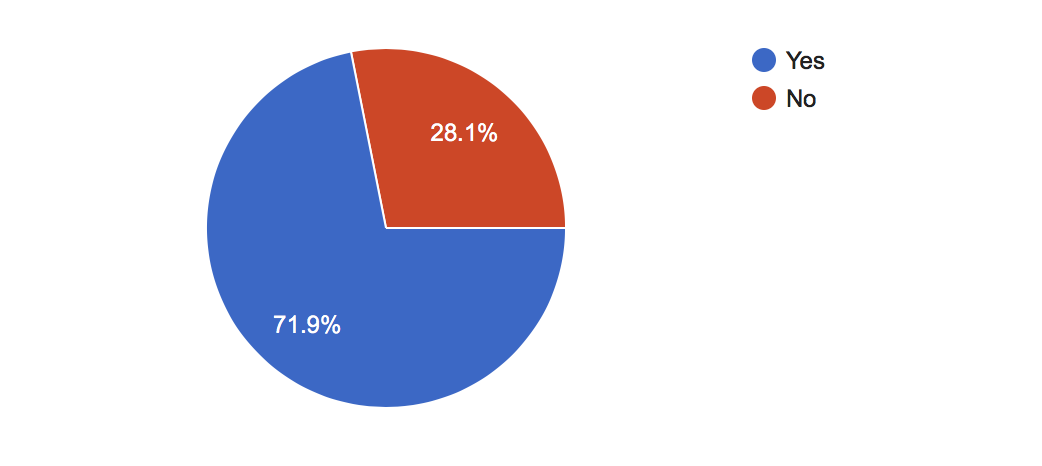
\includegraphics[scale=0.7]{12DoYouLikeServicesThatProduceDigests}
   \caption[Survey Graph about News Digests]{A pie chart showing people's attitudes towards News Digests.}
   \label{SurveyDigests}
\end{figure}

The next question, shown in Figure \ref{SurveyDigests} centred around News Digests\index{News Digests}. Nearly 72\% of respondents said that they liked services that provide news digests.\\

\item \textbf{How often should these news digests be updated?}

\begin{figure}[ht!]
  \centering
    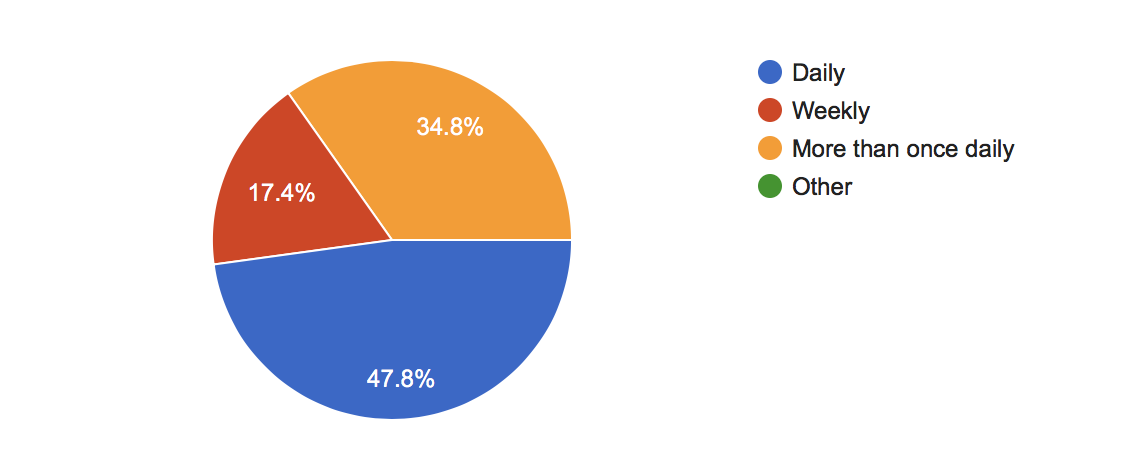
\includegraphics[scale=0.7]{13HowOftenShouldTheseDigestsBeProduced}
   \caption[Survey Graph about News Digests' frequency]{Responses regarding how frequently news digests should be updated.}
\end{figure}

People who were in favour of news digests in general felt that these should be updated at least daily (47.8\%), with a further 34.8\% on top of that saying it should be updated more than once.\\

\item \textbf{What platform should the aggregator be developed for?}

\begin{figure}[ht!]
  \centering
    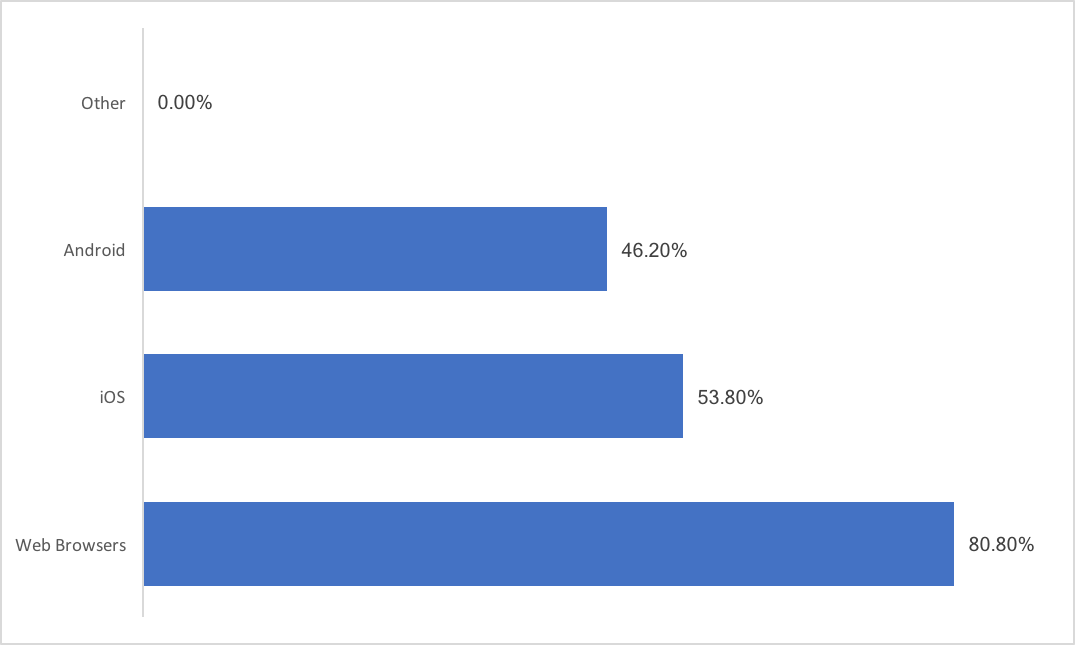
\includegraphics[scale=0.7]{09WhatPlatform.png}
   \caption[Survey Graph concerning potential platforms]{A bar chart showing responses when asked which platform they'd rather see the news aggregator developed for.}
   \label{Survey Platform}
\end{figure}

Finally, respondents were asked which platform they would prefer to see the news aggregator developed for. 80.8\% said they'd want a version for web browsers, and 53.8\% for iOS and 46/2\% for Android. This would suggest that I should develop a web solution and then move to a mobile platform afterwards if there is time.\\

\end{enumerate}
 
\subsection{Related Products}

\subsubsection{Google News}\index{Google!News}

\begin{figure}[H]
  \centering
  \begin{subfigure}{0.8\textwidth}
        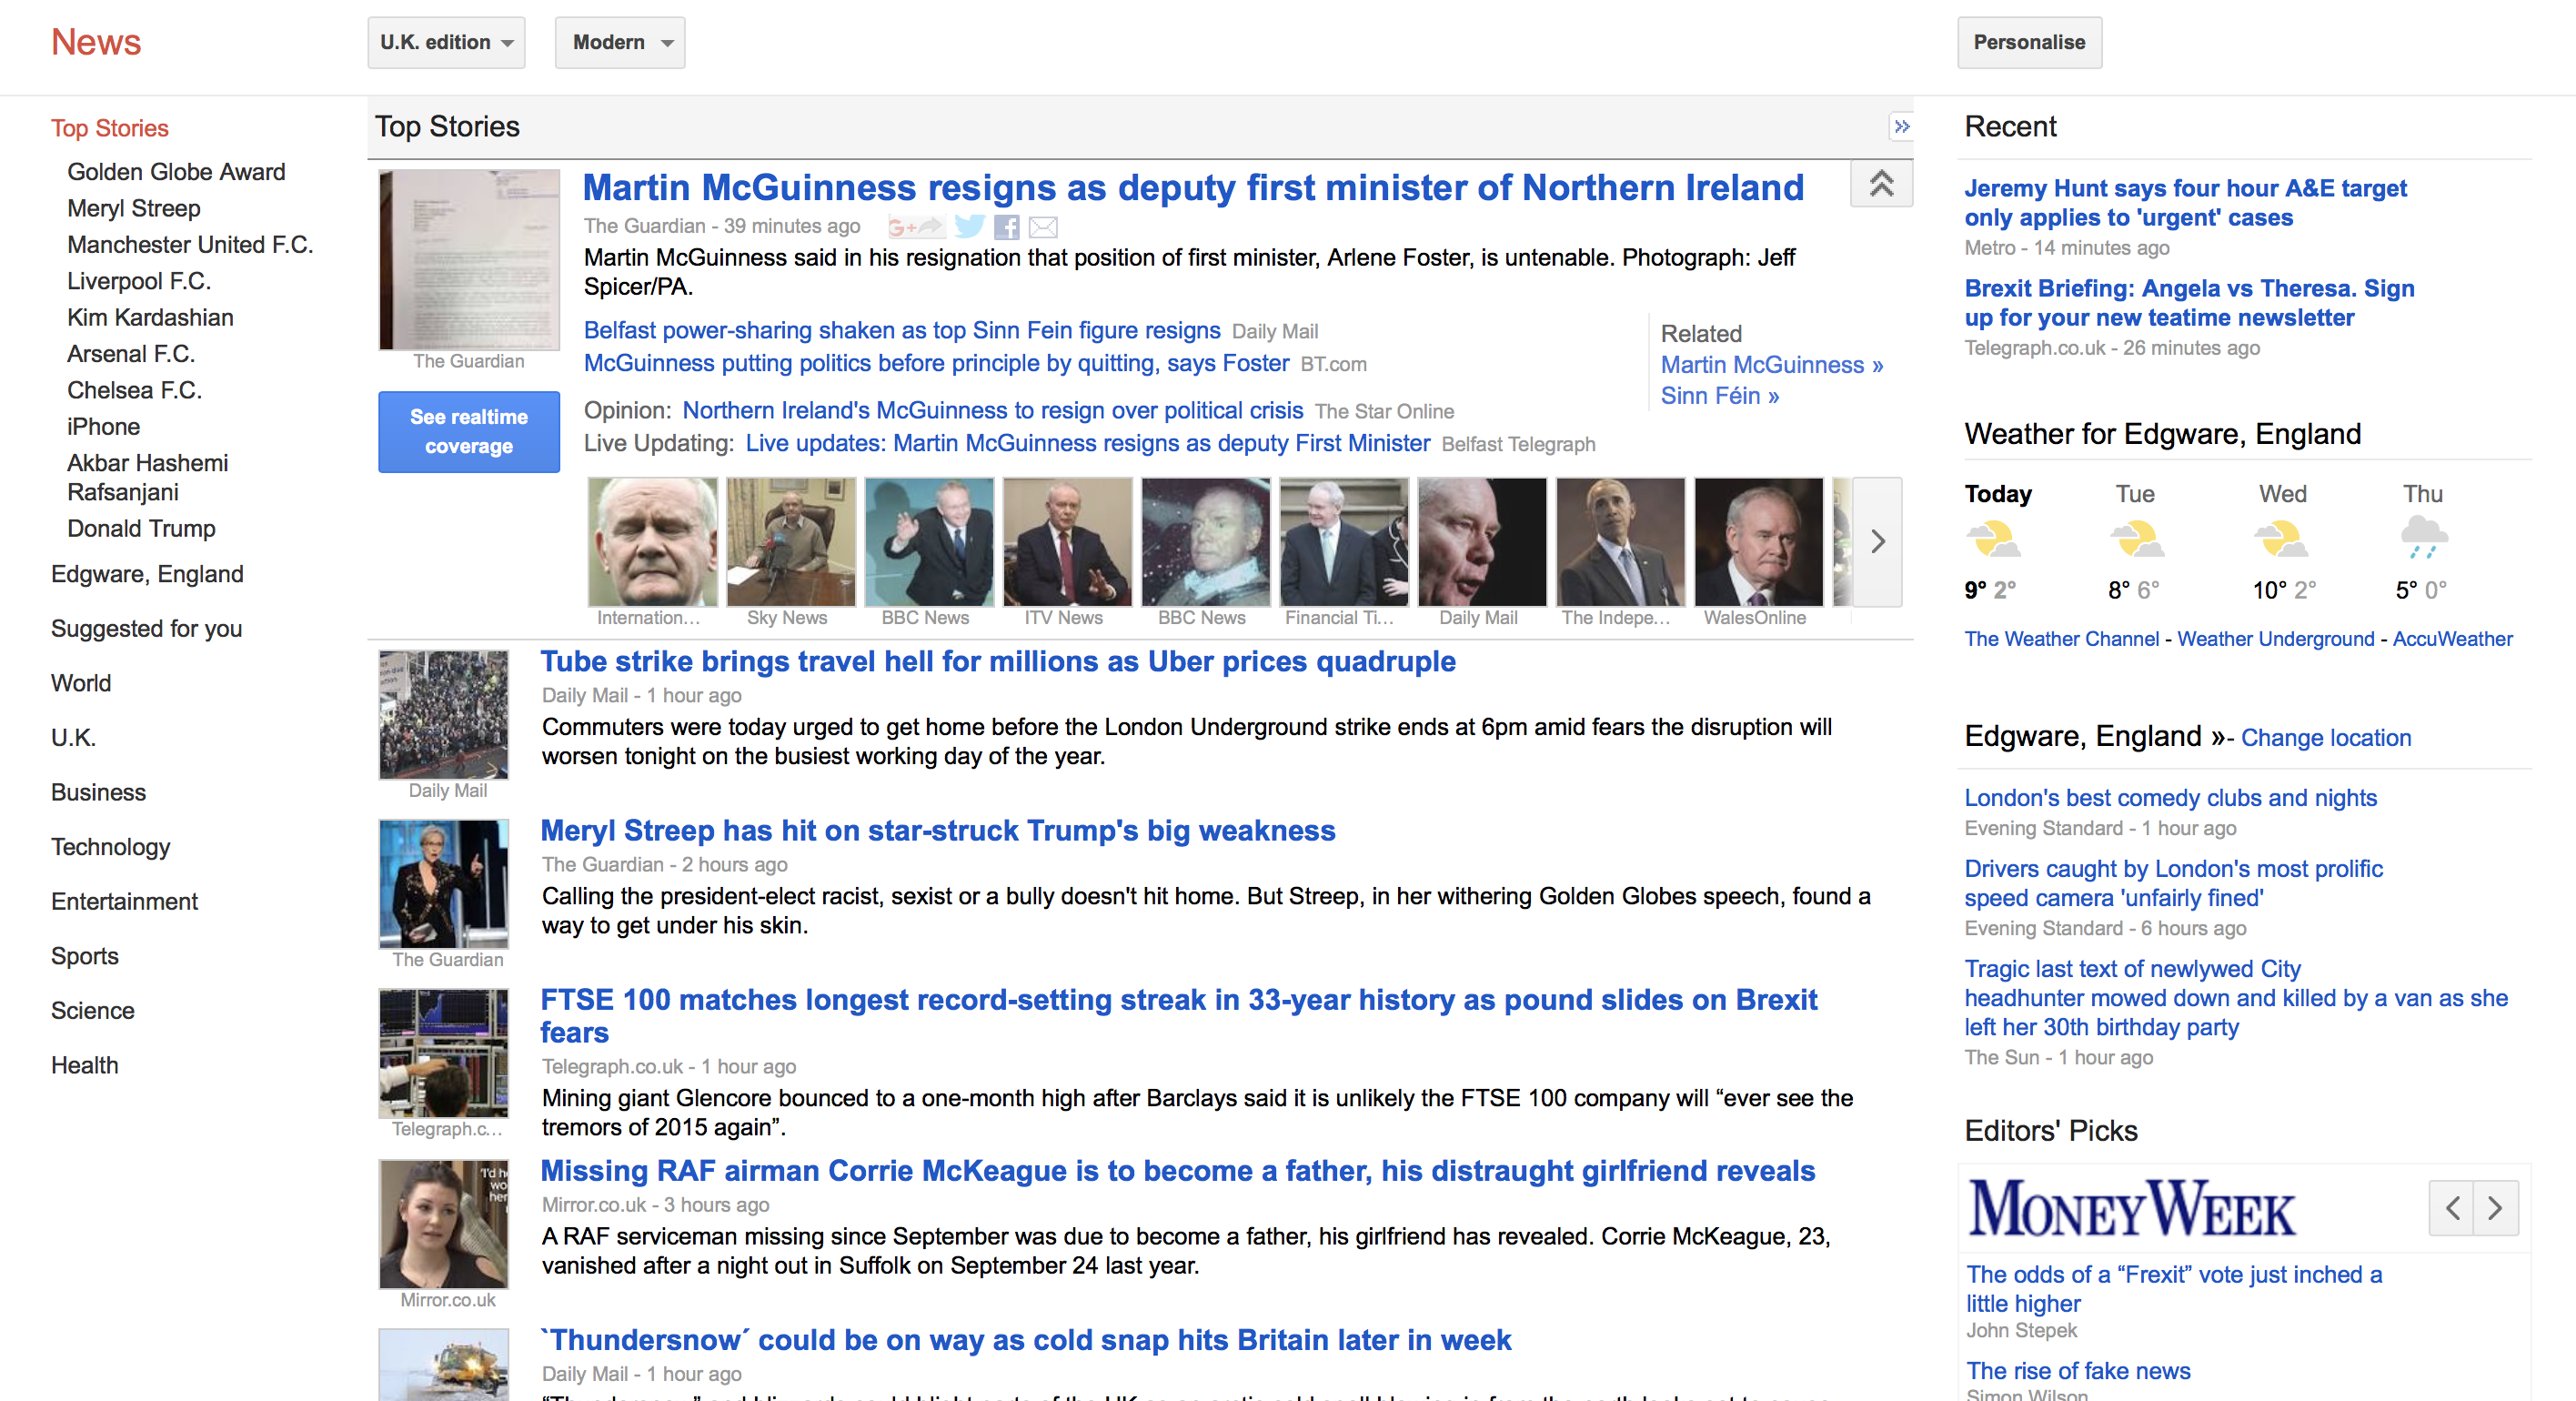
\includegraphics[width=\textwidth]{GoogleHome}
        \caption[Screenshot from the Google News home page]{A section of the homepage for Google News.\cite{googleNews}}
        \label{GoogleNewsHome}
    \end{subfigure}
    
    \begin{subfigure}{\textwidth}
    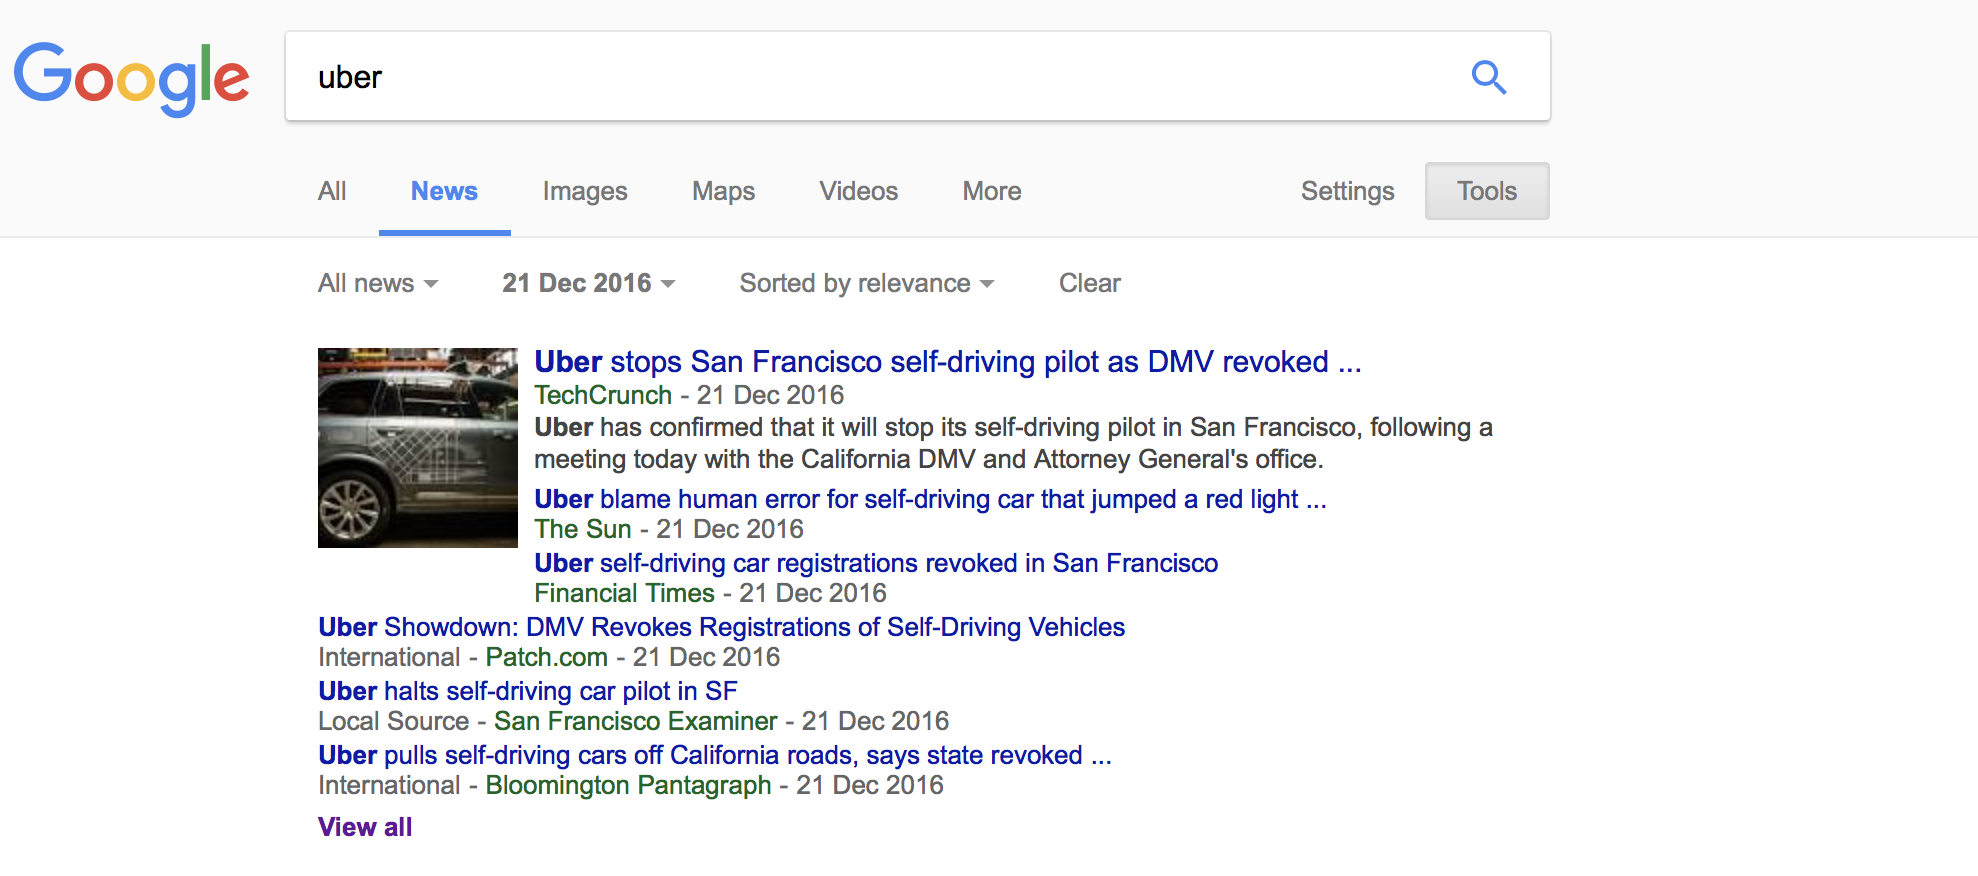
\includegraphics[width=\textwidth]{GoogleUber}
   \caption[Screenshots from a Google News search]{Google News uses clustering techniques to group articles about the same topic together. }
   \label{GoogleNewsUber}
   \end{subfigure}
   \caption[Screenshots from Google News]{Screenshots from Google News}
\end{figure}

Initially developed early in the century and released in 2006, Google News\cite{googleNews} is a free-to-use news aggregator. Google News operates in a similar manner to the traditional Google\cite{google} search engine, thus making it a go to aggregator when searching for a specific topic. Google News also groups "similar" articles together using Clustering\index{Clustering} techniques\cite{googleClustering}. Google News operates purely as a go-between - when clicking on an article the user is taken straight to the media source itself, rather than being able to read the article on Google News itself. 

\subsubsection{Flipboard}\index{Flipboard}

\begin{figure}[H]
  \centering
  \begin{subfigure}[t]{0.3\textwidth}
        
\includegraphics[width=\textwidth]{FlipboardHome.PNG}
        \caption{Users can subscribe to "magazines" that they may be interested in.}
        \label{FlipboardHome}
    \end{subfigure}
    \qquad
    \begin{subfigure}[t]{0.3\textwidth}
    
\includegraphics[width=\textwidth]{Flipboard.PNG}
   \caption{All users are subscribed to \emph{The Daily Edition}, which puts together the latest most popular news.}
   \label{FlipboardDailyEdition}
   \end{subfigure}
   \caption[Screenshots from the Flipboard app]{Screenshots from the Flipboard app}
\end{figure}

Flipboard\cite{flipboard} is a much more recent attempt at a news aggregator (developed in 2010), and relies on the concept of users subscribing to "magazines" on different topics. There's a central "cover page" on the home page that shows the most recent stories from across all a user's subscriptions. Like Google News\index{Google!News}, links from the desktop website send the user to the original media source, while links from within the mobile applications open a browser within the app itself.

\subsubsection{Yahoo News Digest}\index{Yahoo News Digest}

\begin{figure}[ht!]
  \centering
  \begin{subfigure}[t]{0.3\textwidth}
        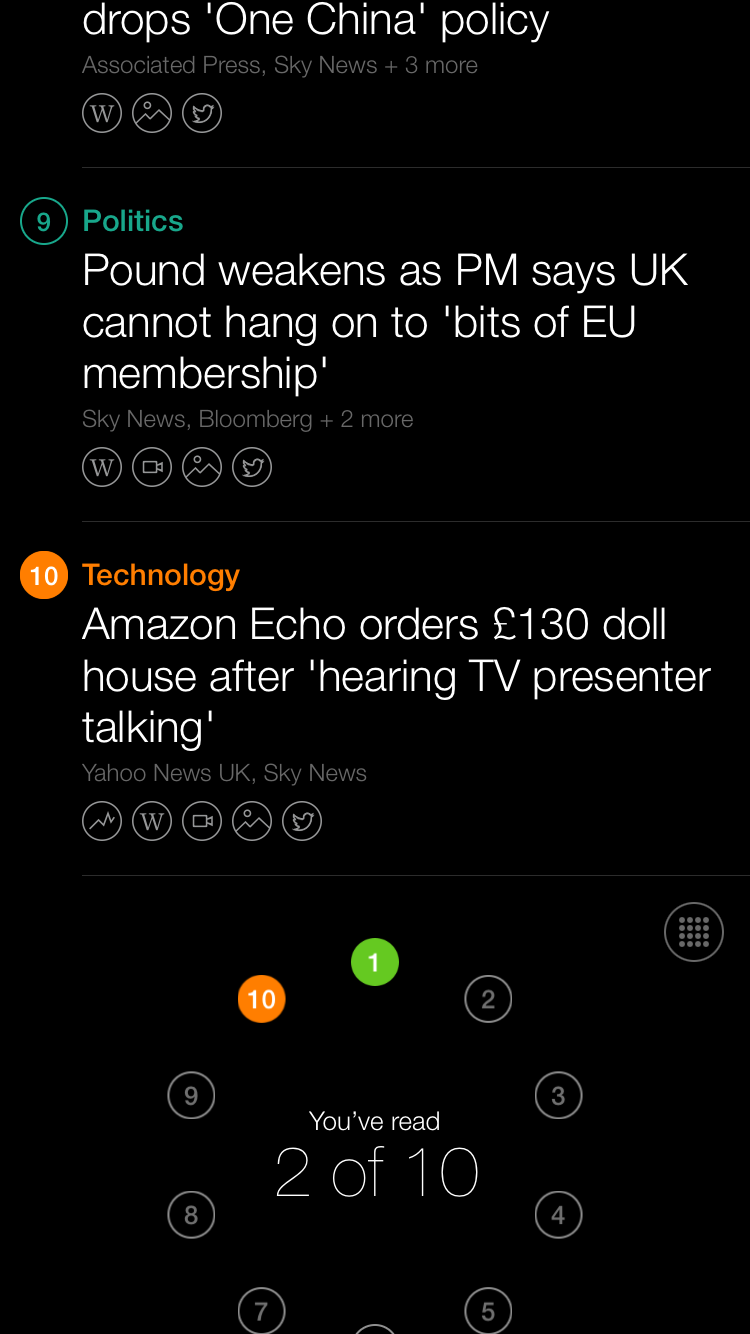
\includegraphics[width=\textwidth]{YNDHome.PNG}
        \caption{A section of the home screen, which displays the top ten stories for the day.}
        \label{YNDHome}
    \end{subfigure}
    \qquad
    \begin{subfigure}[t]{0.3\textwidth}
    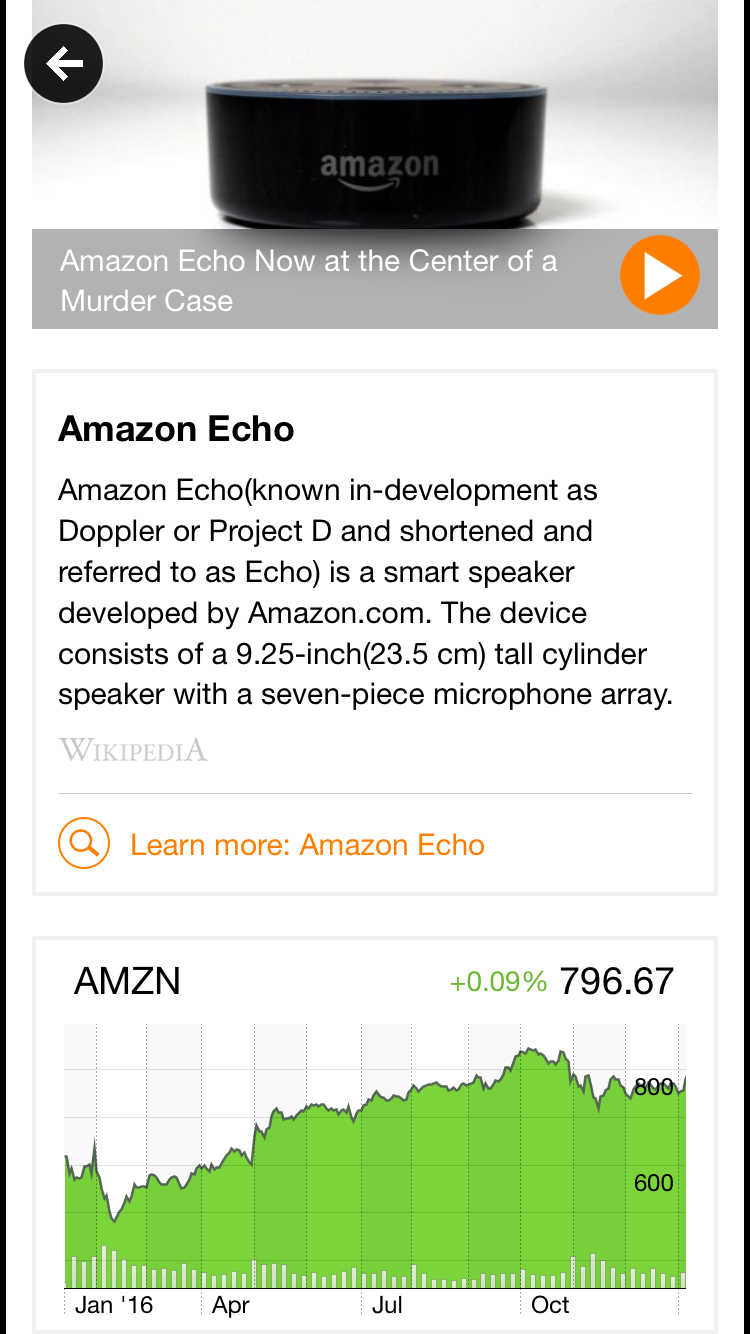
\includegraphics[width=\textwidth]{YNDInfo.PNG}
   \caption{The Yahoo News Digest app provides links and infographics that are relevant to the article.}
   \label{YNDInfo}
   \end{subfigure}
   \caption[Screenshots from the Yahoo News Digest app]{Screenshots from the Yahoo News Digest app\cite{yahooNewsDigest}}
\end{figure}

Yahoo News Digest\cite{yahooNewsDigest} is a direct evolution from Summly\cite{summly}, which was an app that summarised news. Yahoo News Digest is a phone application that creates two digests a day: one in the morning and one in the evening. Each digest contains the ten leading articles from the previous 12 hours. Each article provides a summary of the story and links to relevant other pages - such as articles from Wikipedia\cite{wikipedia}.

\subsubsection{Apple News}\index{Apple!News}

\begin{figure}[ht!]
  \centering
  \begin{subfigure}[t]{0.3\textwidth}
        
\includegraphics[width=\textwidth]{AppleHome.PNG}
        \caption{The home screen for the Apple News app}
        \label{AppleHome}
    \end{subfigure}
    \qquad
    \begin{subfigure}[t]{0.3\textwidth}
    
\includegraphics[width=\textwidth]{AppleSources.PNG}
   \caption{Apple News allows users to select sources and topics to be their favourites.}
   \label{AppleSources}
   \end{subfigure}
   \caption[Screenshots from the Apple News app]{Screenshots from the Apple News app\cite{appleNews}.}
\end{figure}

Apple News\cite{appleNews} is an application that is installed by default on all recent iOS devices. Apple's default attempt at a news aggregator allows users to select their preferred news sources, and from a selection of topics. Apple\cite{apple} then presents on a home screen news from those sources and topics. Clicking on each article keeps it in the native application, rather than sending the user to the media source itself.

\subsubsection{Comparing the existing products}

The existing products are compared in Table \ref{relatedProductsTable} on page \pageref{relatedProductsTable}.

\begin{sidewaystable}
    \begin{tabular}{p{2.5cm}|p{8.75cm}|p{8.75cm}}
    \textbf{Product} & \textbf{What it does well} & \textbf{What it doesn't do well} \\ \hline
    Google News & \tabitem Groups similar articles together & \tabitem Doesn\'t host articles itself - therefore making it harder to navigate than perhaps could be possible. Although, this could be to avoid any copyright issues. \\ & \tabitem Similar to a traditional search engine and so is easy to use\\ & \tabitem Obtains articles instantly, thus providing most up-to-date information when searching  \\ \hline
    Flipboard & \tabitem Provides a home page that allows a user to see the most popular stories at the time related to the user's subscriptions. & \tabitem Topics are much broader than Google News, thus meaning that users can't necessarily search for topics specific-enough for them.\\ & \tabitem Available as a mobile application & \tabitem Flipboard requires registration before being able to read articles \\ \hline
    Yahoo News Digest & \tabitem Yahoo News Digest won the 2014 Apple\index{Apple} Design award\cite{appleDesignAward}\index{Apple!Design award}. & \tabitem There are only ten articles available per digest, and no capability for searching by topic. \\ & \tabitem The articles also provide key infographics, quotes, and other information potentially relevant to the article. & \tabitem Digests are only produced in the morning and the evening, so the news articles presented could be out of date. \\ \hline
    Apple News & \tabitem Allows selection based off both topics and the news sources themselves. & \tabitem Navigation on the application is not simple. If a user has accessed many articles from push notifications, then the user could have to press the back button several times to get back to the home screen.\\ & \tabitem The home screen for the app allows users to see a lot of headlines at a glance. & \tabitem The topics that a user can subscribe to can be quite limited, and aren't reactive to current affairs - for example, if a natural disaster occurs, you couldn't then subscribe to that natural disaster as a topic. \\
  \end{tabular}
  \caption[Related Products in the market and their benefits and drawbacks]{Comparing the relative benefits and drawbacks of Google News, Flipboard, Yahoo News Digest and Apple News}
  \label{relatedProductsTable}
\end{sidewaystable}


\section{Background Research}

\subsection{Machine Learning Techniques}

\subsubsection{Topic Modelling Techniques}\index{Topic Modelling}

\label{TopicModellingTechniques}

Topic modelling is a subsection of Machine Learning\index{Machine Learning} that aims to determine what topic a given document is about. The topics wouldn't be named at this stage, they would simply be given generic names such as Topic A and Topic B. Assigning names to topics will be done at a later stage (see Section \ref{TopicLabelingTechniques}).

\textbf{Latent Semantic Indexing}\index{Latent Semantic Indexing}\index{Topic Modelling!Latent Semantic Indexing}

Also known as Latent Semantic Analysis\index{Latent Semantic Analysis}\cite{lsa}, Latent Semantic Indexing (LSI) was one of the initial forerunners in the field of topic modelling. It uses singular value decomposition to locate patterns in the text of a document and thus form a basis on which to categorise the document. A major benefit of LSI\index{LSI} is that it is fast to train, but in general it has lower accuracy when compared to models that are probabilistic, such as Latent Dirichlet Allocation\index{Latent Dirichlet Allocation}\cite{differenceBetweenLSIAndLDA}.

\textbf{Latent Dirichlet Allocation}

Latent Dirichlet Allocation\index{Latent Dirichlet Allocation} (LDA)\index{LDA}\index{Topic Modelling!Latent Dirichlet Allocation} is a generative probablistic model that assumes that the topic distribution has a Dirichlet prior. The theory behind LDA is that a document of words contains a mixture of different topics, and this is reflected in the final answers given for the algorithm.

\emph{A rough algorithm for performing LDA\cite{ldaExplanation}:}

\begin{enumerate}
	\item \textbf{Set \emph{n} to be the number of topics there are in the document.} We can do this by trial and error. \\
	\item \textbf{Assign every word \emph{w} in the document {d} to a random topic.} These topics are temporary. At this stage we can remove function words, such as "the". However, we keep duplicates - in fact, at this stage they could be in different topics. \\
	\item \textbf{Check and update topic assignments.} To do this, we loop through each word in the document, taking note of how prevalent the word is across documents, and prevalent those topics are in the document. These two probabilities are then passed to a sampling algorithm to generate a new topic for the word. This step is usually completed using the statistical model \emph{Gibbs Sampling}\index{Gibbs Sampling}.
	\item \textbf{Repeat step 3 until there are no more topic-reassignments}. 
\end{enumerate}

\subsubsection{Topic Labelling Techniques}\index{Topic Labelling}

Topic Labelling techniques in the project for labelling the topics that are generated from the LDA analysis of the document in Section \ref{TopicModellingTechniques}. When conducting research into this topic specifically, I found a paper (\emph{Automatic Labelling of Topic Models}\index{Automatic Labelling of Topic Models} by Lau, Grieser, Newman and Baldwin in 2011\cite{topicLabelling}) that documents the creation of an algorithm that labels topics using Wikipedia\cite{wikipedia}\index{Wikipedia} titles. This could work very well in my project, as Wikipedia titles as title headings would allow users to search for topics that are both broad and specific. 

\emph{A rough version of Lau, Grieser, Newman and Baldwin's algorithm:}

\begin{enumerate}
	\item \textbf{Calculate the top 10 topic terms.} This is done by finding the marginal probabilities of each word from the original topic models, and taking the top ten. The marginal probability of a term is the probability of that term being randomly selected given a topic \emph{t}. \\
	\item \textbf{Search Wikipedia\index{Wikipedia} using these terms.} We also search Google\cite{google}\index{Google} using a site restricted search (to Wikipedia) and take the top eight results from each. These are called the \emph{primary labels}. \\
	\item \textbf{Isolate all "noun chunks" from the terms.} In this case noun chunks are combinations of words from the terms that appear next to each other. For example, with the term "Summer Olympic Games" the noun chunks would be "Summer", "Olympic", "Games", "Summer Olympic", "Olympic Games" and "Summer Olympic Games". Note that "Summer Games" is not a noun chunk as the words don't appear juxtaposed. These noun chunks are added to the primary labels from step 2 and are deemed \emph{secondary labels}. \\
	\item \textbf{For each noun chunk:} 
		\begin{itemize}
			\item Check to see if the noun chunk is the title for a Wikipedia article
			\item Remove the noun chunk if it doesn't correspond to a Wikipedia article\\
		\end{itemize}
		
	\item \textbf{Calculate the \emph{Related Article Conceptual Overlap}\index{Related Article Conceptual Overlap} scores.} Related Article Conceptual Overlap (RACO), developed by Grieser et al in 2011\cite{racoCalculation},  is a calculation designed to identify the strength of relationship between terms by inspecting the category overlap between the terms' corresponding articles. We do this for each secondary label still remaining - details on how to calculate the RACO scores are explained in further detail below. \\
	\item \textbf{Discard all secondary labels with RACO\index{Related Article Conceptual Overlap}  score of less than 0.1.} \\
	\item \textbf{Add five highest topic terms to the list.} Now we return to the original list of topic terms from step 1 and add the five highest to the remaining candidates. \\
	\item \textbf{Perform candidate ranking.} There are multiple ways to do this, but the original paper recommends using a variety of statistical methods, based around a T-test, the Chi-squared test and a log-likelihood test. The aim is to estimate how closely related the candidate is to all the terms in the topic. We then take the top candidate as our final answer. \\
\end{enumerate}

\textbf{Calculating the \emph{Related Article Conceptual Overlap}\index{Related Article Conceptual Overlap} }

\emph{Related Article Conceptual Overlap\index{Related Article Conceptual Overlap} } (RACO) was first introduced as a concept in the paper \emph{Using Ontological and Document Similarity to Estimate Museum Exhibit Relatedness}\cite{racoCalculation} \index{Using Ontological and Document Similarity to Estimate Museum Exhibit Relatedness}by Grieser, Baldwin, Bohnert and Sonenberg in 2011. It compares two terms and estimates their similarity by comparing the two terms' similarity on Wikipedia. The core calculation for RACO goes as follows: 
\[Category-Overlap(a,b) = \left|
\left(\bigcup_{p \in O(a)} C(p)\right) \bigcap \left(\bigcup_{p \in O(b)} C(p)\right)\right|
\]

In this equation, \emph{O(a)} represents the outlinks (the links to other articles from the Wikipedia\index{Wikipedia} article) of an article \emph{a} and \emph{C(p)} represents the set of categories that article \emph{p} is a part of.

An issue with the Category-Overlap calculation as it is, is that there's a bias for articles that are larger than others as they will have more outlinks but won't necessarily be in more categories. As a result it's normalised using Dice's coefficient \index{Dice's coefficient} to produce the final RACO equation:

\[sim_{RACO}(a,b) = \frac{2 \times \left|
\left(\bigcup_{p \in O(a)} C(p)\right) \bigcap \left(\bigcup_{p \in O(b)} C(p)\right)\right|}
{\left(\bigcup_{p \in O(a)} C(p)\right) + \left(\bigcup_{p \in O(b)} C(p)\right)}
\]

\label{TopicLabelingTechniques}

\subsubsection{Clustering Techniques}\index{Clustering}

\label{ClusteringTechniques}

Cluster analysis is a machine learning technique that is used to put items that are similar to each other into groups. In practice it's used by Google News\cite{googleNews} to put articles about the same topic together for a user\cite{googleClustering}. There are multiple commonly used types of cluster analysis: \\

\textbf{Centroid Clustering}\index{Centroid Clustering}\index{Clustering!Centroid}

In Centroid Clustering\cite{clusteringWikipedia}, also known as k-means clustering\index{Clustering!k-means}, there are \emph{k} clusters. A vector is calculated for each article in the list. The article is then assigned to the cluster that is closest to it's vector score. A major downside to this method however is that it requires \emph{k} to be defined in advance. In the context of this project, that's not applicable as we don't know how many different articles we are clustering based on. \\

\textbf{Density Clustering}\index{Density Clustering}\index{Clustering!Density}

Density Clustering\cite{clusteringWikipedia} also involves calculating a vector score for each article. Once these have been calculated, they can be graphed, and the areas of the graph that have highest density are chosen as the clusters. An advantage of this over the centroid clustering methods is that we don't need to know the number of clusters beforehand. However, density clustering can become less accurate as it requires areas of sparse density on the graph to precisely separate the different groups, which isn't always possible. \\

\textbf{Hierarchical Clustering}\index{Hierarchical Clustering}\index{Clustering!Hierarchical}

Hierarchical Clustering\cite{hierarchicalClustering}, which is also known as Connectivity Clustering\index{Clustering}\index{Connectivity}, is based on the idea of using distance measures between articles to identify which ones are most similar. There are two approaches to Hierarchical Clustering: 
 \begin{itemize}
 	\item \emph{Agglomerative}\index{Hierarchical Clustering!Agglomerative}, which is a bottom-up approach, assigns each item to its own cluster and then merges pairs that are closer together. 
	\item \emph{Divisive}\index{Hierarchical Clustering!Divisive}, a top-down approach, that begins with all items in a single cluster, and then proceeds to split it into multiple clusters. \\
\end{itemize}

\textbf{Creating a vector score for each item}

The first step in each of the three clustering techniques is to create a vector score for each item. As this will play a big part in the final results, it's important to get this stage right. This can be split into two steps: \\

\begin{enumerate}
	\item \textbf{Find definitive terms within the article.} This can be done using techniques such as the popular \emph{Term Frequency-Inverse Document Frequency}\index{Term Frequency-Inverse Document Frequency}  (TF-IDF)\index{TF-IDF} , which is explained in further detail below. Proper nouns would be useful in this step, as they are more likely to be relevant to what the article is specifically about. \\
	\item \textbf{Create a vector.} This vector, based from the definitive terms from the first step, would be a set of keywords and corresponding weights. \\
\end{enumerate}

\textbf{Term Frequency-Inverse Document Frequency}\index{Term Frequency-Inverse Document Frequency}

TF-IDF\cite{tfidf} is designed to identify terms that appear frequently in one article that don't occur a lot over the entire set of articles (also known as the \emph{corpus}). Variations of it are commonly used by search engines to identify search results that are most relevant to a query. The calculation for TF-IDF is as follows: \\

\emph{Term Frequency}\index{Term Frequency-Inverse Document Frequency!Term Frequency}

Term Frequency can be most simply calculated as the frequency of a term in a document. However, this could result in a bias towards terms that appear in longer articles. A more accepted way to calculate the Term Frequency therefore is to use a normalising function, called augmented frequency:

\[tf(t,d) = 0.5 + 0.5 \times \frac{f_{t,d}}{max\{f_{t',d} : t' \in d\}} \] \\

\emph{Inverse Document Frequency}\index{Term Frequency-Inverse Document Frequency!Inverse Document Frequency}

Inverse Document Frequency is used to check in how many documents of a corpus \emph{D} a given term \emph{t} occurs. It is an inverse function, so as to minimise the value for the term when it is common amongst various different documents. It is also logarithmically scaled. It is calculated using the following formula:

\[idf(t,D) = \log{\frac{\left|D\right|}{\left|d \in D : t \in d\right|}} \] \\

\emph{Term Frequency-Inverse Document Frequency}\index{Term Frequency-Inverse Document Frequency}

\[tfidf(t,d,D) = tf(t,d) \times idf(t,D)\] 

\subsection{Summarisation Techniques}       

Summarisation\index{Summarisation} techniques will be (predictably) used for summarising the merged articles that were identified by the processes of Topic Modelling \index{Topic Modelling}, Topic Labelling\index{Topic Labelling} and Clustering\index{Clustering}. There are two types of summarisation: 

\begin{itemize}
	\item \textbf{Extractive Summarisation}\index{Summarisation!Extractive}, which consists of taking sentences that are important from the original text, and discarding the rest.\cite{extractiveTechniques}
	\item \textbf{Abstractive Summarisation}\index{Summarisation!Abstractive}, which aims to generate a piece of text using natural language techniques. A key to this is that some words in the final summary may not have been the original piece of text.
\end{itemize}

\subsubsection{Extractive Summarisation Techniques}

\label{extractiveSummarisation}

\textbf{LexRank and TextRank}\index{LexRank}\index{TextRank}

There are two well known examples of extractive summarisation: LexRank and TextRank.

LexRank and TextRank have very similar methods for extracting a summary\cite{lexRank}. Initially a graph is constructed, that consists of one node for each sentence in the corpus. Then a clustering algorithm is applied, using a TF-IDF\index{TF-IDF} calculation to determine similarities. 

There are a couple of key differences between LexRank and TextRank. The first arises in the calculation. Both use a TF-IDF calculation, but they are varied slightly. LexRank uses a cosine similarity function in order to weight the final calculation, whereas TextRank uses a more simple logarithmic weighting to perform the calculation. 

Both use Google's famous PageRank\index{PageRank} algorithm to then rank the importance of each sentence based on the calculations in the previous step. With \emph{d} being a damping factor, the PageRank of a node \emph{u} is given as:

\[p(u) = \frac{d}{N} + (1-d)\sum_{v \in adj[u]}\frac{p(v)}{deg(v)} \] 

After this has been calculated, the top ranked sentences are taken by the TextRank algorithm to form the summary. However, in the LexRank algorithm sentence position and length are also taken into consideration. Also, when adding a sentence to the summary, the LexRank checks the sentence against the summary to ensure that it won't be redundant. As a result of this extra step, LexRank is considered more suitable than TextRank when summarising multiple documents, whereas TextRank is only normally used for summarising a single document.

\subsubsection{Abstractive Summarisation Techniques}\index{Summarisation!Abstractive}

There are six common methods for abstractive summarisation, which can be split evenly into two distinct categories\cite{abstractiveTechniques}. These two categories centre around the creation of a representation of the given document: \\

\begin{itemize}
	\item \textbf{Structure based methods} consist of techniques that involve determining the important information in a document by considering its structure\cite{abstractiveTechniquesOriginal}. Ways of doing this include fitting the given document to a template, or converting the text in a tree-like structure. \\
	\item \textbf{Semantic based methods} involve building a semantic representation of the given document and then feeding that into an algorithm that generates natural language that forms the final summary. \\
\end{itemize}

\textbf{Structure based summarisation} \\

\emph{Tree based summarisation}\index{Summarisation!Tree based}

With tree based structuring, the first step is to create a dependency tree to represent the document. A dependency tree\index{Dependency Tree} is a tree with a node for each word in a sentence, the links between the trees show which words depend on each other. For example, given the sentence \emph{This is an example}, we can construct a tree as in figure \ref{dependencyTree}:

\begin{figure}[ht!]
  \centering
    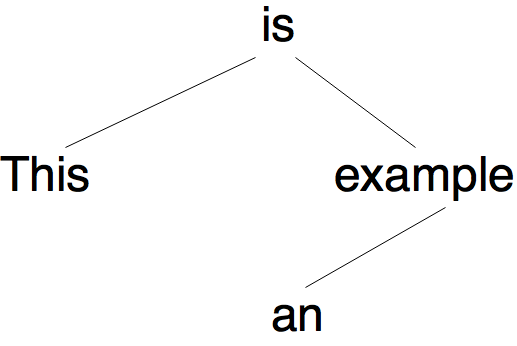
\includegraphics[scale=0.4]{DependencyTree.png}
   \caption[An example of a Dependency Tree]{A possible dependency tree for the sentence \emph{This is an example}}
   \label{dependencyTree}
\end{figure}

In the tree (figure \ref{dependencyTree}), the word \emph{This} is dependent on \emph{is} and so is linked. \emph{an} is linked to \emph{example} in a similar way, and \emph{an example} is dependent on the verb \emph{is} and so also has a link to it. 

Once dependency trees have been created for each of the sentences a similarity algorithm is used to find sentences that are similar. The common phrases between these similar sentences are then taken and form the basis of the final summary. A language generator then combines the common phrases and arranges it to create a final set of summary sentences.

An obvious disadvantage to this method is that if only common phrases are taken from the sentences, context could be lost from some of the sentences. However, on the other hand, the use of a language generator means that a more coherent, more grammatically correct summary is formed. \\

\emph{Rule based summarisation}\index{Summarisation!Rule based}

In rule based summarisation\cite{ruleBasedSummarisation}, the process is centred around a list of pre-determined categories. With each of these categories, there is a pre-determined set of questions to be answered. 

For example, with a theoretical category \emph{Product Launch} we could have the following questions:

\begin{enumerate}
	\item What is the name of the product?
	\item What company is launching it?
	\item What type of product is it?
	\item What's new about it?
	\item What price is it retailing at?
\end{enumerate}

This represents only a subset of the possible questions we could have for this category.

To perform rule based summarisation, the first step is to analyse the document and determine which category it fits best. Once that's been determined, the next stage is to analyse the text to find answers to the questions corresponding to that category. These answers are then fed in to a natural language generator that forms sentences, and thus the summary.

Results for this method of abstractive summarisation have been promising, but the method has a major disadvantage in that the list of categories and questions needs to be pre-determined. As a result, it might not be an optimal algorithm to use for the ever-changing world of news reporting. \\

\emph{Ontology based summarisation}\index{Summarisation!Ontology based}

Methods of ontology based summarisation have been developed, primarily using domain based ontology. In this method a "domain expert" defines a domain ontology for a news event. Each new document is then classified into a topic using these domain ontologies\index{Domain Ontology}. Important phrases are determined by how close they are to items in the ontology. These phrases are then passed into a natural language generator to form the final summary sentences.

A key disadvantage to this method is that a lot of the domain ontologies has to be manually determined by the "domain experts" and so can be very time consuming. As a result this may also not be particularly optimal for summarisation of news events. \\

\textbf{Semantic based summarisation} \\

\emph{Multimodal Semantic summarisation}\index{Summarisation!Multimodal Semantic}

Multimodal semantic summarisation can work on documents that contains both text and images. First, a semantic model is built to represent the document. This model is made up of different concepts that are surmised from the text. For example, the sentence \emph{Multimodal Semantic summarisation is an example of an algorithm that performs abstractive summarisation}\index{Summarisation!Abstractive} could form the concept shown in figure \ref{multimodalSummarisation}:

\begin{figure}[ht!]
  \centering
    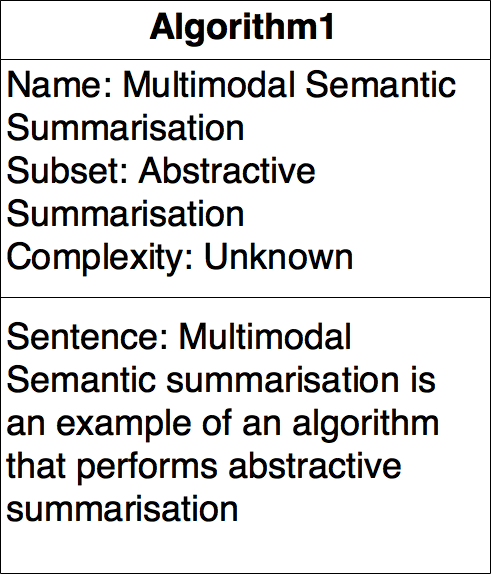
\includegraphics[scale=0.3]{MultimodalSummarisation.png}
   \caption[A concept created during multimodal semantic summarisation]{A possible concept created from the analysis of the sentence \emph{Multimodal Semantic summarisation is an example of an algorithm that performs abstractive summarisation}}
   \label{multimodalSummarisation}
\end{figure}

Concepts\index{Concept!Multimodal Summarisation} are gradually filled with more information as the entire text is analysed. Links are also added between concepts that share some relationship. For example in figure \ref{multimodalSummarisation} if there was another sentence that surmised a concept called \emph{Abstractive Summarisation} then there would be a link from \emph{Algorithm1} to that new concept. 

The next step is to rank the concepts. This is done by taking into account the completeness of the concept, and the number of links that the concept as to others. This way, the concepts are ranked by which is most important to the original document. Once the key concepts have been identified summary sentences can be generated featuring these concepts. \\

\emph{Information Item based method}\index{Summarisation!Information Item}

Information Item based summarisation\cite{informationBasedSummarisation} relies on the content of the summary being determined from an abstract representation of the original document, rather than the sentences from the document themselves. To do this, the document is first scanned so that Information Items (InIt) can be generated. An information item is defined as being "the smallest element of coherent information in a text or sentence". 

Once the information items have been created, they are then ranked using frequency analysis to find the most important predicates and entities from the original document. This step is near identical to the term frequency stage in extractive summarisation (Section \ref{extractiveSummarisation})\index{Summarisation!Extractive}. These information items that are ranked highly are then combined and fed into a natural language generator to form the final summary sentences. \\

\emph{Semantic Graph summarisation}\index{Summarisation!Semantic Graph}

Semantic Graph summarisation centres around a rich semantic graph (RSG)\index{Rich Semantic Graph}. The document is first converted into a RSG. Each node in the RSG represents a noun or verb in the document, and the links between the nodes represent the semantic and topological relations between these nouns and verbs. In the second stage, heuristic rules are used to reduce the semantic graph to a more minimalistic version. This will form the basis of the final summary. In the final step, the minimised RSG is passed into a generator that creates the final summary sentences.

The steps are outlined in the flowchart provided in figure \ref{semanticGraphSummarisation}.

\begin{figure}[ht!]
  \centering
    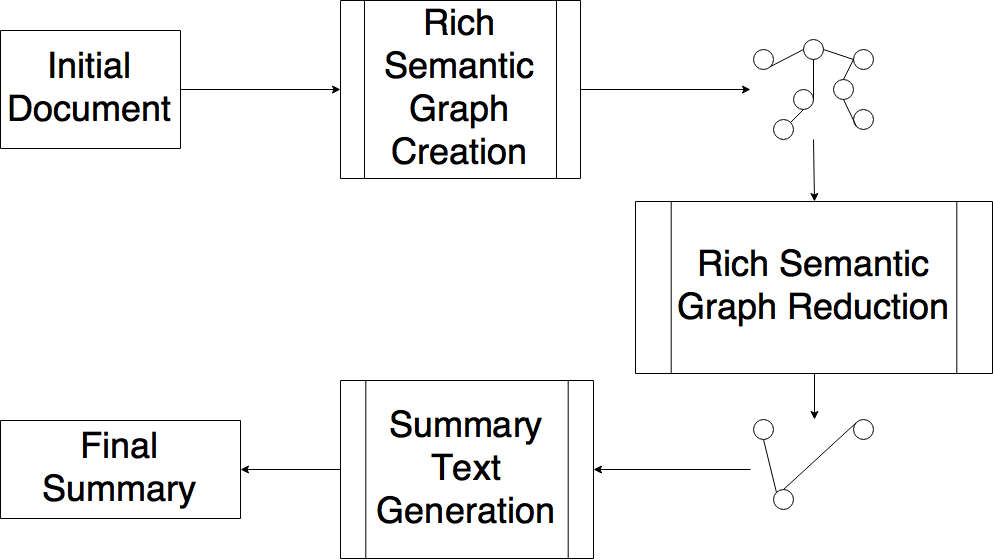
\includegraphics[scale=0.4]{SemanticGraphSummarisation.png}
   \caption[A flowchart showing the process of semantic graph summarisation]{This shows the process of semantic graph summarisation in a flowchart based on those provided in \cite{abstractiveTechniques, abstractiveTechniquesOriginal}}.
   \label{semanticGraphSummarisation}
\end{figure}

Semantic Graph summarisation has had success with producing an abstractive summary that has fewer redundant sentences, and is also good at producing grammatically correct sentences. However, it's only designed for use with a single document as input. As a result it might not be suitable as a method for summarising the multiple documents needed for the aggregator, unless it's combined with another method.

\subsection{Potentially Useful APIs}

\subsubsection{News Outlets}\index{News!Outlets}

\textbf{Readership statistics for selected outlets in the United Kingdom\index{United Kingdom}}

Statistics below are taken from the \emph{Digital News Report 2016}\cite{digitalNewsReport}\index{Digital News Report} by the Reuters Institute for the Study of Journalism\cite{reutersInstitute}\index{Reuters Institute for the Study of Journalism}. Viewership is given as a percentage of people who say they use the outlet at least weekly.

\begin{table}[H]
	\centering
	\begin{tabular}{l|c|r}
		\textbf{Outlet} & \textbf{Viewership} & \textbf{Political Stance} \\ \hline
		BBC\index{BBC} & 51\% & Neutral \\ \hline
		Mail Online\index{Mail Online} & 17\% & Right \\ \hline
		Huffington Post\index{Huffington Post} & 14\% & Left \\ \hline
		The Guardian & 14\% & Left \\ \hline
		Sky News Online\index{Sky News} & 11\% & Neutral \\ \hline
		The Telegraph Online\index{Telegraph, The} & 9\% & Right \\ \hline
		The Independent\index{Independent, The} & 6\% & Centrist \\ \hline
	\end{tabular}
	\caption[Readership statistics for selected UK outlets]{Readership statistics for selected outlets in the United Kingdom}
	\label{viewershipFigures}
\end{table}

\textbf{\\The Guardian\cite{guardian}}

\emph{The Guardian}\index{Guardian, The} is a UK newspaper that commands about 14\% of the viewership as outlined in Table \ref{viewershipFigures}. It is also known for having an API that allows a user full and free access to all articles, including the article text itself. The API can access any article dated on or after 1999, and as long as not used for a commercial purpose, is completely free to use. 

To obtain an article from \emph{The Guardian} there are two calls that need to be made. First, we make a call to the search endpoint, which returns a JSON object similar to this:

\begin{lstlisting}[language=json, firstnumber=1]]
{
    "response": {
        "status": "ok",
        "userTier": "free",
        "total": 1,
        "startIndex": 1,
        "pageSize": 10,
        "currentPage": 1,
        "pages": 1,
        "orderBy": "newest",
        "results": [
            {
                "id": "politics/blog/2014/feb/17/alex-salmond-speech-first-minister-scottish-independence-eu-currency-live",
                "sectionId": "politics",
                "sectionName": "Politics",
                "webPublicationDate": "2014-02-17T12:05:47Z",
                "webTitle": "Alex Salmond speech - first minister hits back over Scottish independence - live",
                "webUrl": "https://www.theguardian.com/politics/blog/2014/feb/17/alex-salmond-speech-first-minister-scottish-independence-eu-currency-live",
                "apiUrl": "https://content.guardianapis.com/politics/blog/2014/feb/17/alex-salmond-speech-first-minister-scottish-independence-eu-currency-live"
            }
        ]
    }
} 
\end{lstlisting}

From this, we extract the apiUrl, and call this, with the API key in the request headers. This will return the raw text for the article. \\

\textbf{The Financial Times}\index{Financial Times, The}

\emph{The Financial Times} is an internationally renowned, UK based broadsheet that provides news primarily on politics and the financial sector. Their API is similar to that of \emph{The Guardian}, but with a key difference that could prove very useful. While \emph{The Guardian} allows a user to query the API by date, \emph{The Financial Times} does better. It has a notification endpoint, which allows a user to query with a specific date and time. They are then returned a list of "notifications", showing articles that have been created, updated or deleted since the time provided, as shown in the example below.

\begin{lstlisting}[language=json, firstnumber=1]]
{
  "requestUrl": "http://api.ft.com/content/notifications?since=2014-05-06T10:00:00.000Z",
  "notifications": [
    {
      "type": "http://www.ft.com/thing/ThingChangeType/UPDATE",
      "id": "http://www.ft.com/thing/7348edd8-0403-11de-845b-000077b07658",
      "apiUrl": "http://api.ft.com/content/7348edd8-0403-11de-845b-000077b07658"
    }
  ],
  "links": [
    {
      "href": "http://api.ft.com/content/notifications?since=2014-05-06T18:42:35.000Z",
      "rel": "next"
    }
  ]
}
\end{lstlisting}

Using this, the notifications of type UPDATE are kept, and we query for the raw data using the apiUrl in a similar fashion to before in the example for \emph{The Guardian}\index{Guardian, The}. \\

\textbf{News API}

A major issue is that most newspapers (for example, \emph{The New York Times}\cite{newYorkTimes}\index{New York Times}) only give the first paragraph to an article in their API, and don't give out their full articles as standard. There are solutions, such as Webhose\cite{webhose}\index{Webhose}, that offer feeds into this outlets, but at either a cost, or with a very limited number of requests per month. 

News API\cite{newsApi}\index{News API} is a company that provides an API to get headlines for over seventy different news outlets. A call returns data in the JSON format as follows:

\begin{lstlisting}[language=json, firstnumber=1]
{
"status": "ok",
"source": "the-next-web",
"sortBy": "latest",
"articles": [
{
	"author": "Abhimanyu Ghoshal",
	"title": "Are these ridiculous headphones the way forward for music tech?",
	"description": "All the amazing tech we now have at our disposal for enjoying music is closing us off from other people instead of bringing us together. Is there hope yet?",
	"url": "https://thenextweb.com/gear/2017/01/26/can-music-tech-make-us-sociable-again/",
	"urlToImage": "https://cdn3.tnwcdn.com/wp-content/blogs.dir/1/files/2017/01/Vinci-hed-1.jpg",
	"publishedAt": "2017-01-26T13:12:10Z"
}
]
}
\end{lstlisting}

We can use the url provided for each of these results to get to the webpage of the corresponding article. However at this stage I'll need to create a scraper to extract the raw content of the article. There could be copyright implications for this step, even though the final production summary won't look the same as the raw content. These implications will be fully examined in the final report.

News API counts amongst its 70 sources the following: \\

\begin{itemize}
	\item BBC News \index{BBC}
	\item Mail Online \index{Mail Online}
	\item \emph{The Telegraph} \index{Telegraph, The}
	\item \emph{The New York Times} \index{New York Times}
	\item Associated Press \index{Associated Press}
	\item \emph{The Independent} \index{Independent, The}
	\item \emph{The Daily Mirror} \index{Daily Mirror, The} \\
\end{itemize}

News API also has \emph{The Financial Times}\index{Financial Times, The} and \emph{The Guardian}\index{Guardian, The}, although these are left off the list above as they have their own fully accessible APIs.  

\subsubsection{Wikipedia}

Wikimedia\index{Wikimedia} (the parent company for Wikipedia\cite{wikipedia}) provides documentation for the Wikipedia\index{Wikipedia} API on its website MediaWiki website. Here, I can search using the search term that a user has used (perhaps in searching for a topic), and get a result that is as follows:

\begin{lstlisting}[language=json, firstnumber=1]
{
    "query": {
        "searchinfo": {
            "totalhits": 4152
        },
        "search": [
            {
                "ns": 0,
                "title": "Albert Einstein",
                "snippet": "&quot;<span class=\"searchmatch\">Einstein</span>&quot; redirects here. For other uses, see <span class=\"searchmatch\">Albert</span> <span class=\"searchmatch\">Einstein</span> (disambiguation) and <span class=\"searchmatch\">Einstein</span> (disambiguation). <span class=\"searchmatch\">Albert</span> <span class=\"searchmatch\">Einstein</span> (/?alb?rt ?a?n?ta?n/; German:",
                "size": 124479,
                "wordcount": 13398,
                "timestamp": "2015-05-10T12:37:14Z"
            },
            ...
}
\end{lstlisting}

The search query can be altered to provide different information, such as the URL for the lead image, which can be used to show previews of various items to users. The Wikipedia API can also be used in the topic labelling aspect of the Machine Learning techniques (see Section \ref{TopicLabelingTechniques}).

\newpage

\section{Project Plan}

\subsection{What needs to be done}

\label{whatNeedsToBeDone}

The project can be split into three sections:

\begin{enumerate}
	\item Machine Learning and summarisation aspects
	\item Back End server
	\item Front end application(s) \\
\end{enumerate}

\subsubsection{Machine Learning and Summarisation aspects}

\label{machineLearningSummarisationPhases}

This stage will provide the implementation for taking in articles, identifying their topics, clustering them, and summarising them. This can therefore be split into three phases as such:

\begin{enumerate}
	\item Topic Modelling\index{Topic Modelling} and Topic Labelling\index{Topic Labelling} of an article
	\item Clustering\index{Clustering} of articles
	\item Summarisation\index{Summarisation} of articles in a cluster \\
\end{enumerate}

\subsubsection{Back End Server}

This aspect of the project will have two key functions:

\begin{enumerate}
	\item Provide articles to the Machine Learning functions of the project.
	\item Provide a set of API methods for the front end application(s) that perform the functions a user may require, described in more detail in the front end section. \\
\end{enumerate}

\subsubsection{Front end application(s)}

The front end application(s) will need to consist of the following core features:

\begin{itemize}
	\item Search for specific topics
	\item Subscribe to specific topics
	\item View summarised articles
	\item Create and view news digests \\
\end{itemize}

Initially this should be completed on one platform, and if time permits, this could be extended to another platform.

\subsection{Milestones and fallbacks}

Each phase described in section \ref{whatNeedsToBeDone} can be a milestone. However, for the project to be deemed a success there are minimal requirements:

\subsubsection{Machine Learning and Summarisation aspects}

It's easy to say that all aspects of this (section \ref{machineLearningSummarisationPhases}) will be required to make a success of the project. In this case, a minimal requirement, in my opinion, would be for Phase 1 (Topic Modelling\index{Topic Modelling} and Topic Labelling\index{Topic Labelling}) and Phase 2 (Clustering\index{Clustering}) to be fully complete, along with some form of extractive summarisation\index{Summarisation!Extractive} for Phase 3. An ideal scenario would be to have an abstractive summarisation solution\index{Summarisation!Abstractive}, or even a combination of extractive and abstractive solutions. As a result of this, it would be wise to initially create an extractive solution for Phase 3, as it would then provide a good fallback in case the ideal scenario doesn't pan out.

\subsubsection{Back End Server}

Both phases of the back end will need to be fully functional, as the other aspects of the project depend on it. Phase 1 should not be particularly difficult to implement however, and phase 2 (API methods for the front end) can be built in conjunction with the front end, and so can adapt to progress on that front.

\subsubsection{Front end application(s)}

All phases of the front end should be available, with the possible exception of the creation and viewing of news digests\index{News Digests}, for the project to be deemed a success. At the very least, a skeleton application should be created that provides these features. As extensions, with more time, the UI can be spruced up to provide a good user experience, and then the application could also potentially be extended to new platforms.

\subsection{Road Maps}
 
\begin{figure}[ht!]
  \centering
    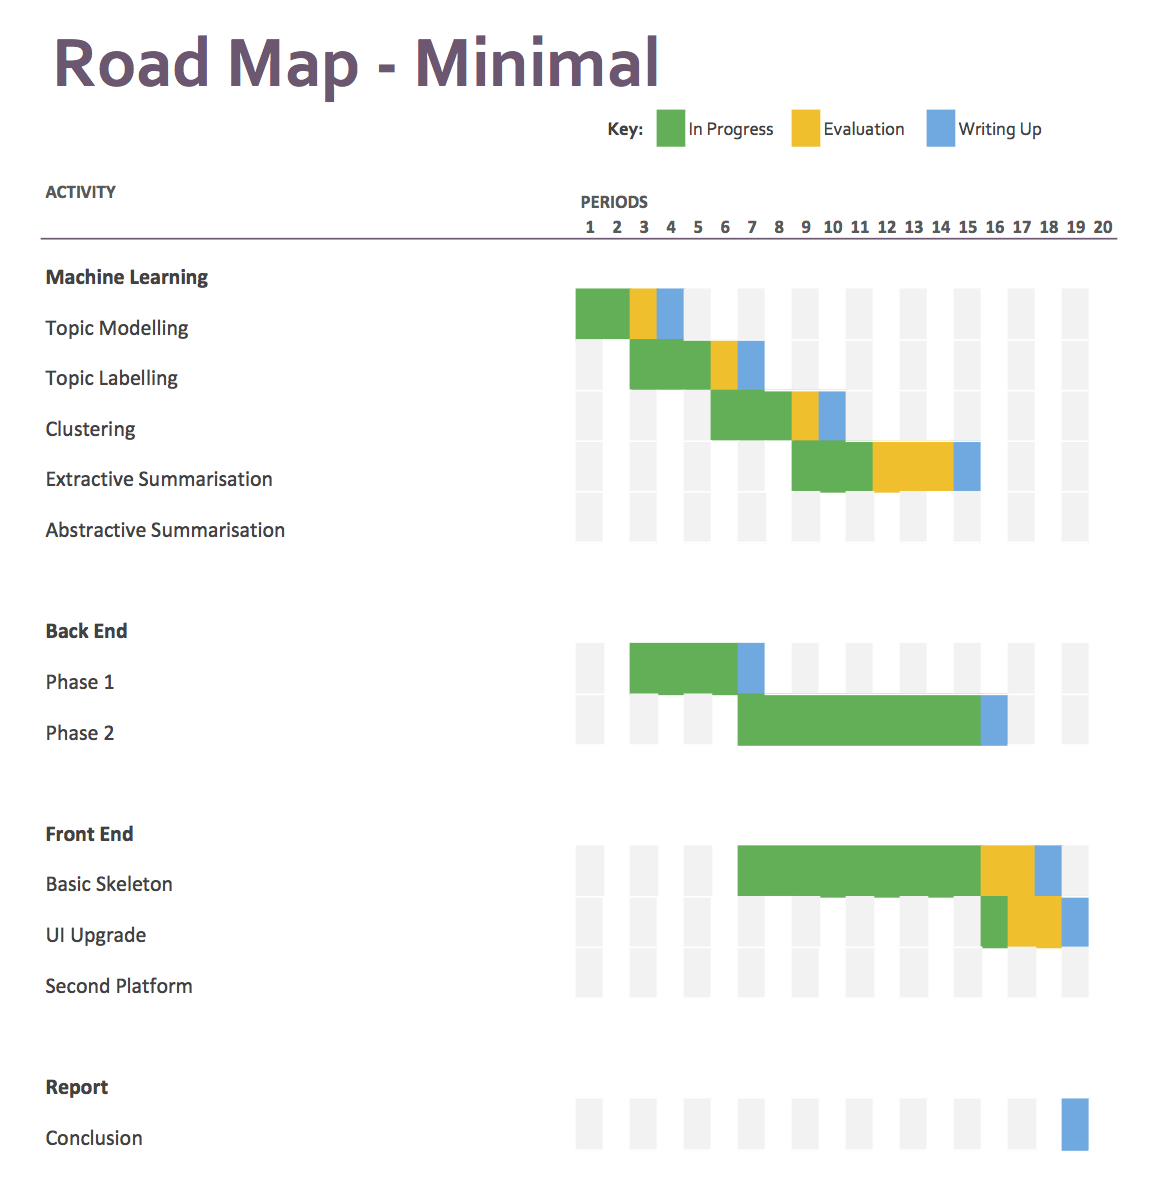
\includegraphics[scale=0.8]{MinimalRoadMap.png}
    \caption[A minimal road map]{This is a Gantt chart representing the minimal road map for my project. Each period corresponds to one week between now and the final deadline for the project.}
\end{figure}

\begin{figure}[ht!]
  \centering
    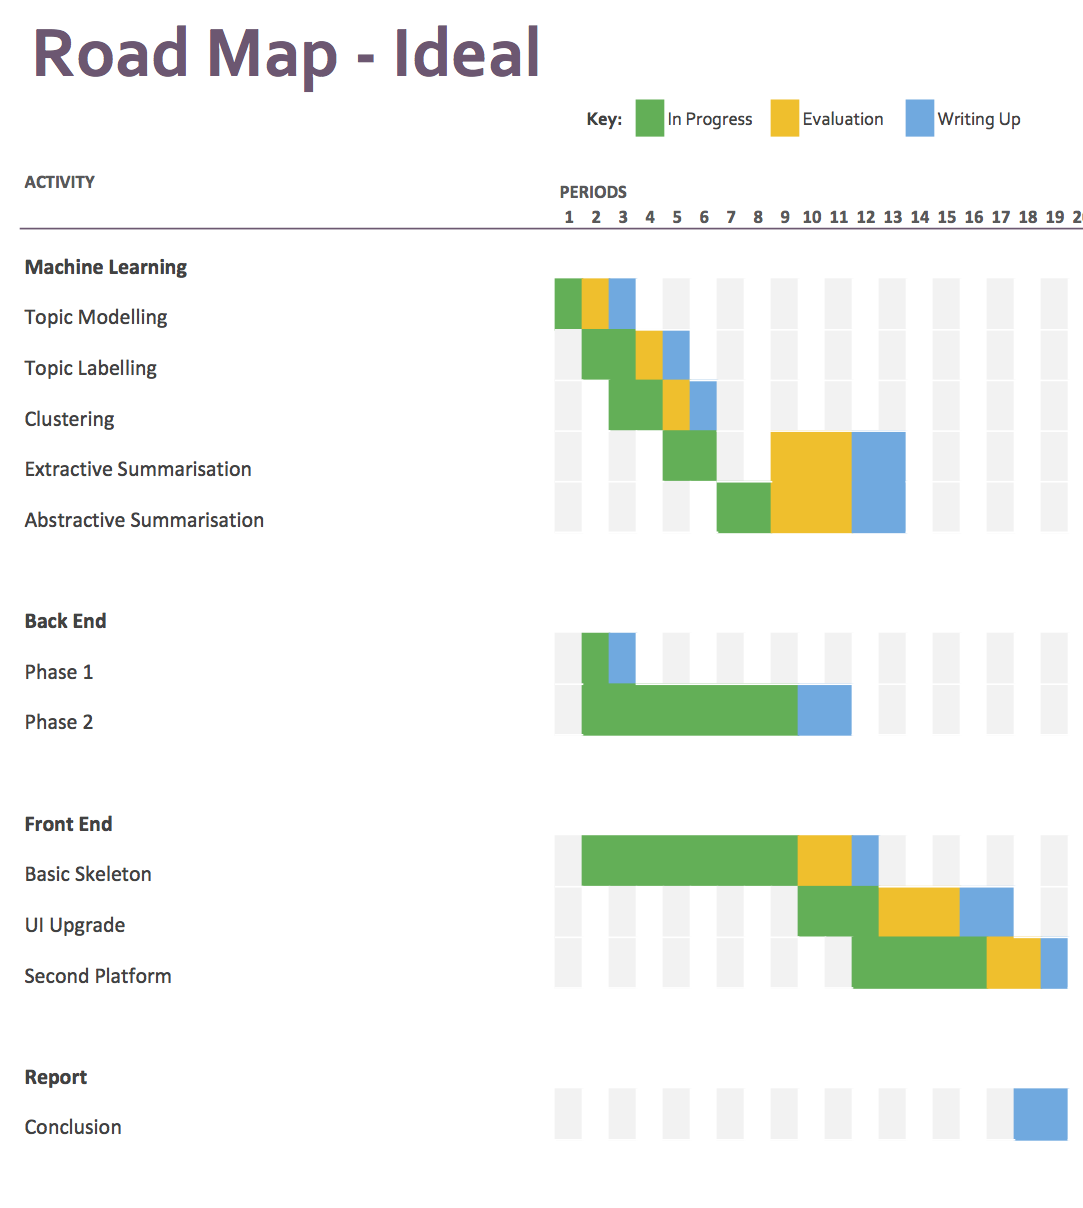
\includegraphics[scale=0.8]{IdealRoadMap.png}
    \caption[An ideal road map]{This is a Gantt chart representing the ideal road map for my project. Each period corresponds to one week between now and the final deadline for the project.}
\end{figure}

\clearpage

\section{Evaluation Plan}

There are two key aspects that need to be tested in the evaluation of the project:

\begin{enumerate}
	\item Summarisation of articles
	\item The front end application
\end{enumerate}

\subsection{Evaluating the summarisation}

When evaluating the summarisation\index{Summarisation}, there are two items that need to be checked. First of all, has the topic been correctly identified? Secondly, is the summarisation presented an accurate depiction of the original article? The evaluation of the topic itself can be done myself initially, and then once summarisation has been completed a good marker for success would be with a user survey.

In this user survey, the user would be presented with an article (or multiple articles) and the summaries. Based on how much of the summarisation plan is actually completed, this aspect of the survey would vary. If both an abstractive\index{Summarisation!Abstractive} and extractive\index{Summarisation!Extractive} algorithm exist, then the user can be presented with a summary from each. Here the user can be asked two (or possibly three) questions:

\begin{enumerate}
	\item On a scale from 1 to 5, how good is this summary for the corresponding article?
	\item Do you feel this summary misses any key information?
	\item \emph{(If multiple summaries are presented.)} Which summary do you think most accurately and fully reflects the article provided?
\end{enumerate}

Question one can be used to evaluate each summary, and thus evaluate the summarisation algorithm that's been used. Question three can then be used to select the best algorithm for the final version of the project. Questions one and two would be designed to evaluate the actual success of summarisation in the project. Since summarisation is an important aspect of the project, a score of 3 out of 5 (60\%) would be classed as adequate in my opinion. Average scores of 4 out of 5 or higher should be the aim for the project to be deemed a success.

With the evaluation completed as a user survey\index{User!Survey}, and without the need for a front end, this part of the evaluation can actually be completed as soon as the summarisation algorithms have been completed, and so are listed in the road map as to be done in parallel with the front end development.

\subsection{Evaluating the front end}

The front end is a bit trickier to evaluate than the summarisation, but can still largely be achieved with the help of a survey.

The key aspects in this section would be to evaluate:

\begin{itemize}
	\item Searching for specific topics
	\item Subscribing to specific topics
	\item Viewing summarised articles
	\item Creating and viewing news digests \\
\end{itemize}

For each of the listed aspects there are two questions: Is it intuitive (can it be done without needing help), and does it work as expected.

To evaluate this, I will provide the application to a focus group, and ask them to do the following:

\begin{enumerate}
	\item Search for Tim Cook (Apple CEO)
	\item Subscribe to Tim Cook\index{Cook, Tim}
	\item Find and read a recent article about Tim Cook
	\item View a daily digest for Tim Cook
	\item Repeat the process for a topic of their choice \\
\end{enumerate}

For each step the user will be asked:

\begin{itemize}
	\item Did you require assistance to perform this task?
	\item Could this process have been made easier? How?
\end{itemize}

A truly intuitive application would mean that the answer to both these questions would be no in every case. The application can therefore be deemed a large success if this is the case. In practice, I will deem the application to be a success if there is a 80\% success rate.

Another aspect of evaluating the front end would be the evaluation of the user interface. For this, I will take advantage of the Undergraduate Fair, by providing the application to visitors, and asking them for feedback on the user interface and the application in general. A fair like this would be more suited to general feedback, as visitors will be viewing many projects in a short space of time.

\newpage

\section{Design}

\subsection{Front End Architecture\index{Front End}\index{Architecture} Diagram}

\begin{figure}[H]
  \centering
    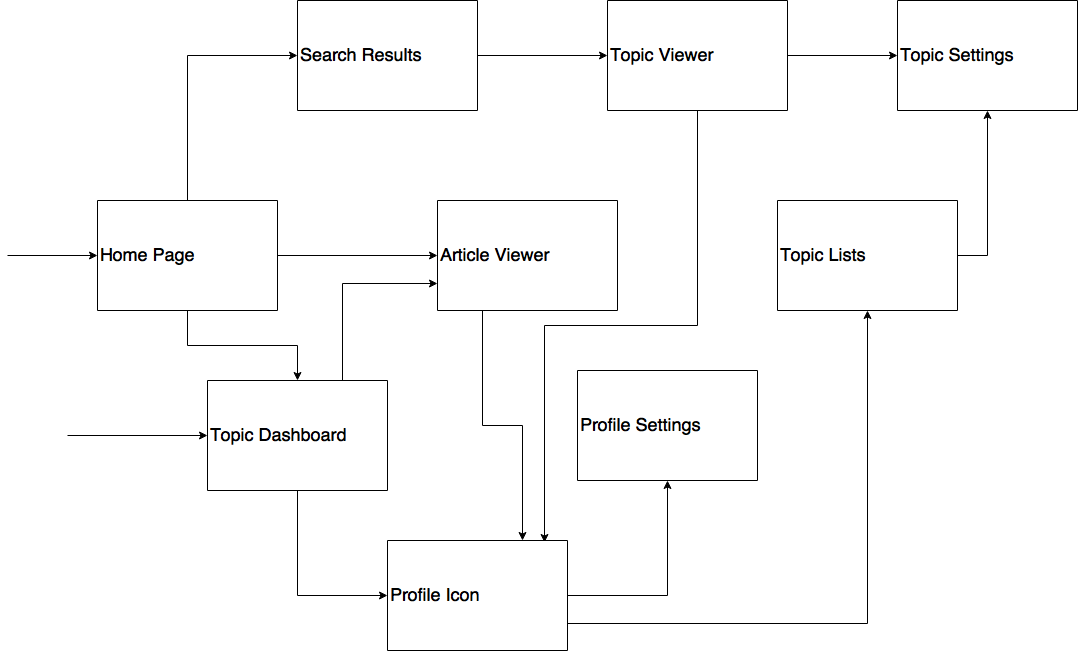
\includegraphics[scale=0.4]{FrontEndArchitecture.png}
   \caption[A basic diagram of the expected architecture of the front end]{This diagram doesn't show all anticipated connections between each facet of the application's front end. For example, the profile icon is in theory accessible anywhere when the user is logged in.}
   \label{frontEndArchitecture}
\end{figure}

\subsection{User Story}

\subsubsection{Home Page}

If a user has not logged in, the first page they will see on opening to the website will be the Home Page. The key to the design of the home page is that it's easy to get started for a user. They are presented with a large search box that they can use without having to sign in. There'll also be a row of trending articles displayed below the search bar. This row will consist of icons consisting of images and titles below, as shown in the wireframe\index{Wireframe}. There's a navigation bar at the top, that is present on all screens, with a button to register and a button to sign in on the top right, and a link to information about the application itself on the top left.

\begin{figure}[ht!]
  \centering
    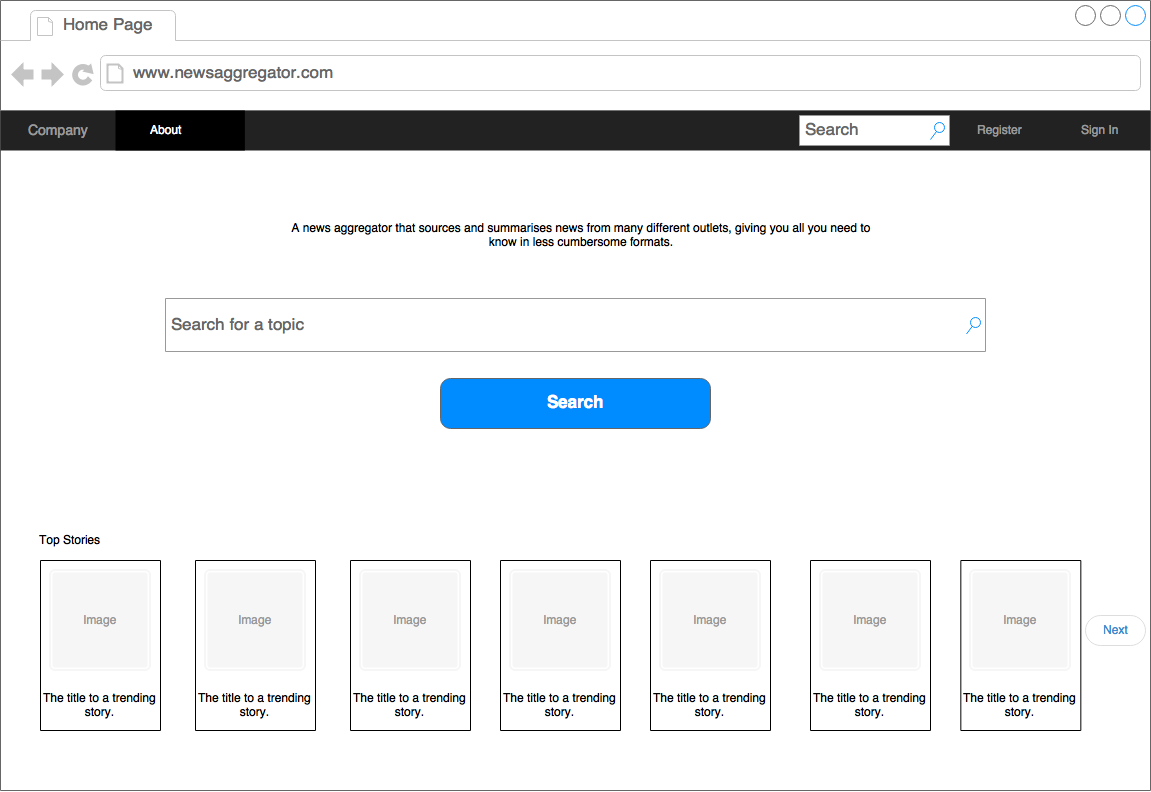
\includegraphics[scale=0.3]{HomePage.png}
   \caption[A wireframe of the Home Screen]{A key focus of the home page is that the user can easily search for articles without having to sign in or register.}
   \label{homePage}
\end{figure}

\subsubsection{Topic Dashboard}

For a user that is logged in, or alternatively a user that has logged in (or signed up) from the home page will first see the topic dashboard screen that shows sets of articles corresponding to each topic they are subscribed. For users who don't have any topics that they are subscribed to, they will instead go back to the home page. The topic dashboard initially shows leading articles from across all the topics they are subscribed to. They can drag to one direction (akin to a sideways swipe on a phone or tablet) to see articles pertaining to the next topic. 

Articles themselves are presented as panels. On a panel is an image for the article, with the title overlaid. In the top right hand corner are icons corresponding to the sources that the article has been summarised from. Leading articles (those out of the most recent that have the most sources attached) are placed in the larger panels on the top left and bottom right of the screen, as shown in the diagram.

\begin{figure}[ht!]
  \centering
    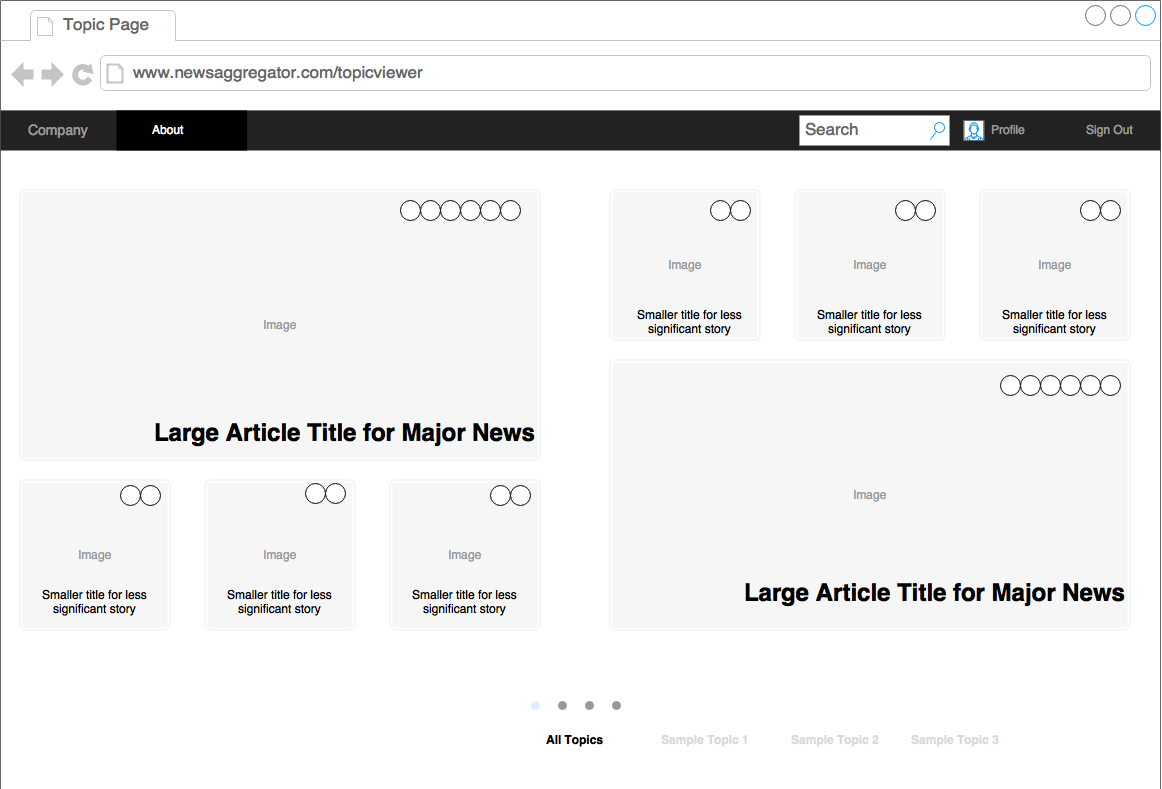
\includegraphics[scale=0.3]{TopicDashboard.png}
   \caption[A wireframe of the Topic Dashboard]{The topic dashboard has the ability to show articles across all topics, or pertaining to a specific topic.}
   \label{topicDashboard}
\end{figure}

\subsubsection{Search Results Page}

The search results page is designed to allow users to see as much as possible and do as much as possible without having to leave the page. The results are presented in the application's panel design, with an image corresponding to each panel. Below the panel, is a description of the topic, that is likely to be created from the first paragraph of the Wikipedia\cite{wikipedia}\index{wikipedia} article about that particular topic. Below this are two buttons, one to view the topic's articles, which will go to a topic viewer page (shown later), and a subscribe button. If logged in, the user is taken to the topic settings page, where they can choose any particular preferences they have for this specific topic. If the user isn't logged in, they are taken to a page allowing them to log in or register, before being taken to the preference page.

It's necessary at this stage to have a user sign in if they want to subscribe to a topic. This way, they can access their topics from anywhere. In addition to this, the search bar is still prominent on the search results page, so that users can edit their queries easily in case of minor errors.

\begin{figure}[ht!]
  \centering
    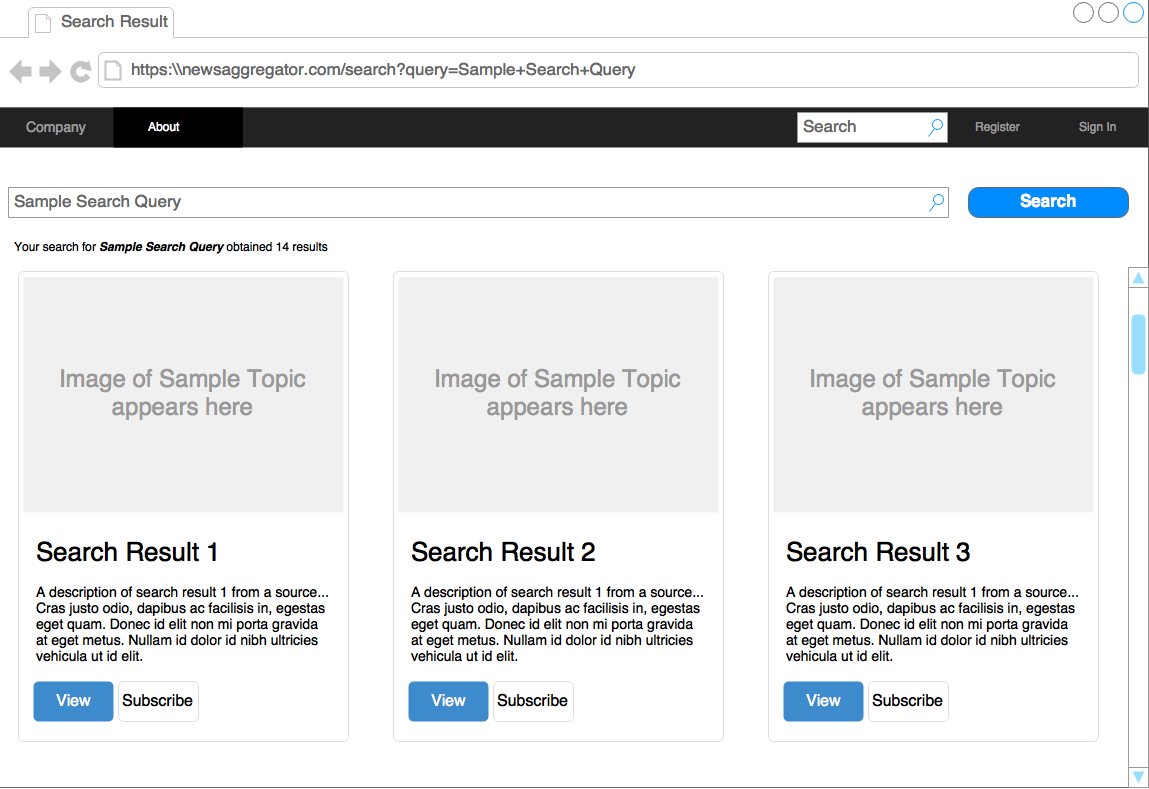
\includegraphics[scale=0.3]{SearchPage.png}
   \caption[A wireframe of the Search Results page]{The Search Results page has a focus on showing users as much information as possible about each topic.}
   \label{searchPage}
\end{figure}

\subsubsection{Topic Viewer}

The topic viewer is accessed if a user has clicked on the view button from the search results page. This screen is similar to that of the topic dashboard. Minor changes include the page control at the bottom of the screen being replaced by page statistics, including figures about how often articles are created, the number of subscribers, and the total number of hits that the page has had. The other major difference is the presence of a subscribe button in the top right hand side of the screen. As with the search results page, this leads to the topic preferences screen if logged in, and to a page prompting a user to sign in or register when not already logged in.

The remaining aspects of the screen are the same - namely the panelled articles, and the icons in the top right of each panel that indicate which sources the article originated from.

\begin{figure}[ht!]
  \centering
    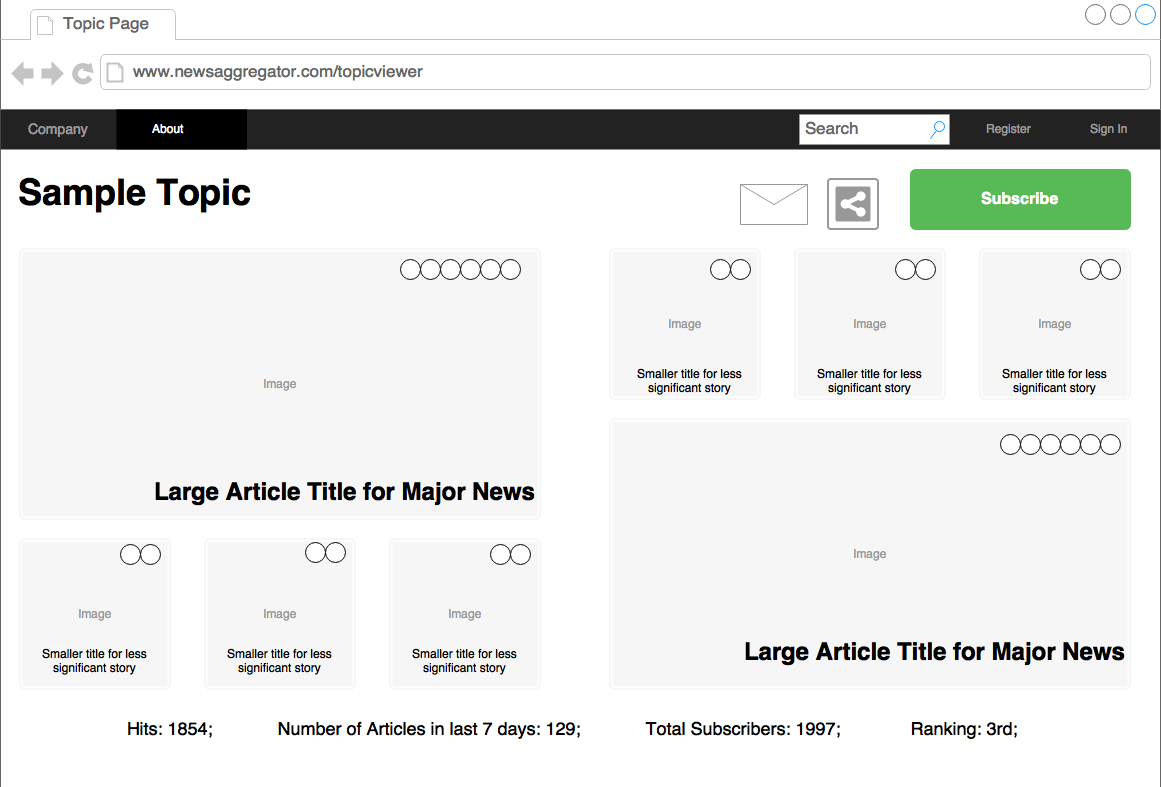
\includegraphics[scale=0.3]{TopicViewer.png}
   \caption[A wireframe of the Topic Viewer]{The topic viewer is similar in structure to the topic dashboard, but with the addition of statistics and a subscribe button.}
   \label{topicViewer}
\end{figure}

\subsubsection{Topic Settings}

The aforementioned Topic Settings page sets out two preferences from the user for a specific topic. These are namely: \\

\begin{itemize}
	\item \textbf{Should the topic's articles be included in the user's email digest?}
	
	This is answered by a simple on/off switch. \\
	
	\item \textbf{Which sources should be used to construct summaries}
	
	This aspect is done using the panelling effect used in other screens. Each news outlet's logo forms the basis of the panel, with the title of the outlet below. These panels form buttons that the user can click on to either select or deselect an outlet. The panel will either have a coloured outer rim, or an embedded effect to indicate selection. \\
\end{itemize}

\begin{figure}[ht!]
  \centering
    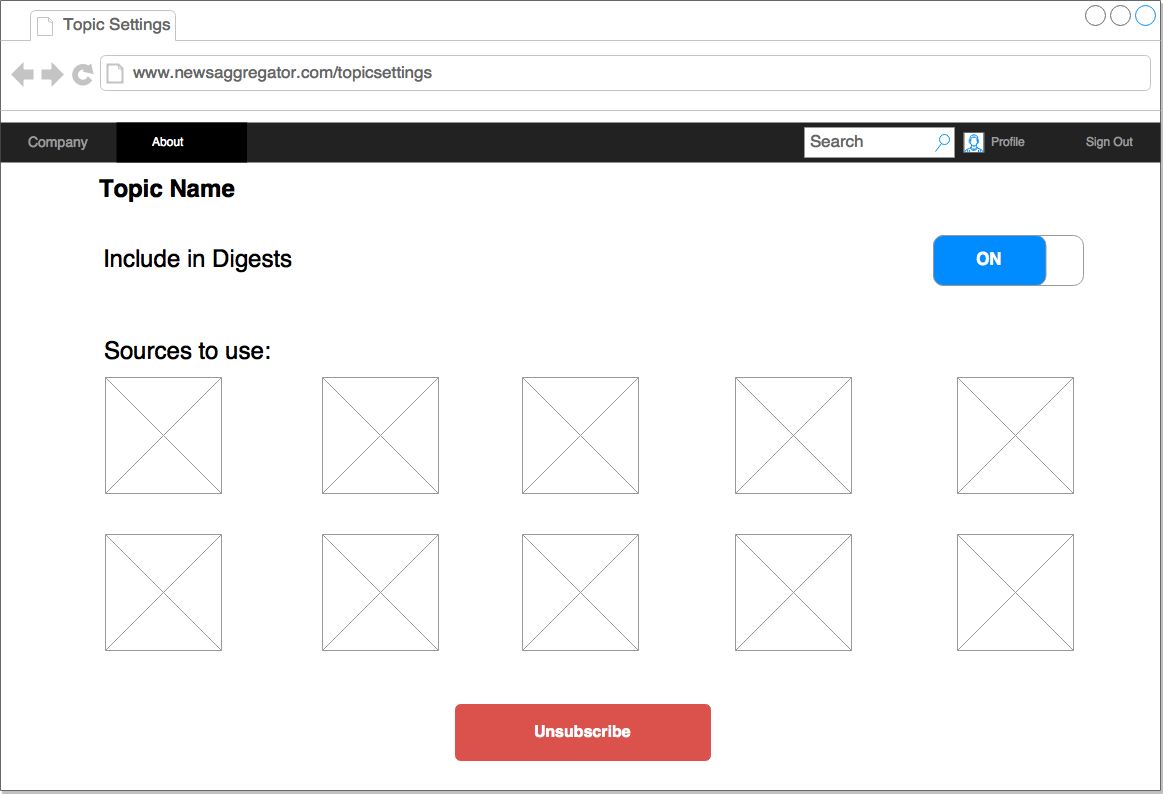
\includegraphics[scale=0.3]{TopicSettings.png}
   \caption[A wireframe of the Topic Settings page]{The Topic Settings page allows users to specify key preferences about the topic.}
   \label{topicSettings}
\end{figure}

\subsubsection{Article Viewer}

When the user clicks on an article panel in the topic viewer or topic dashboard they are presented with the summarised article itself. This screen is modelled on standard news interfaces, and produces the headline, image and article body on the left hand side of the page. On the right hand side are links to the original articles that the summary was generated from, and links to other articles that are in the same topic. 

Like most other screens in the application, there is also a share button on the top right, and an email button.

\begin{figure}[ht!]
  \centering
    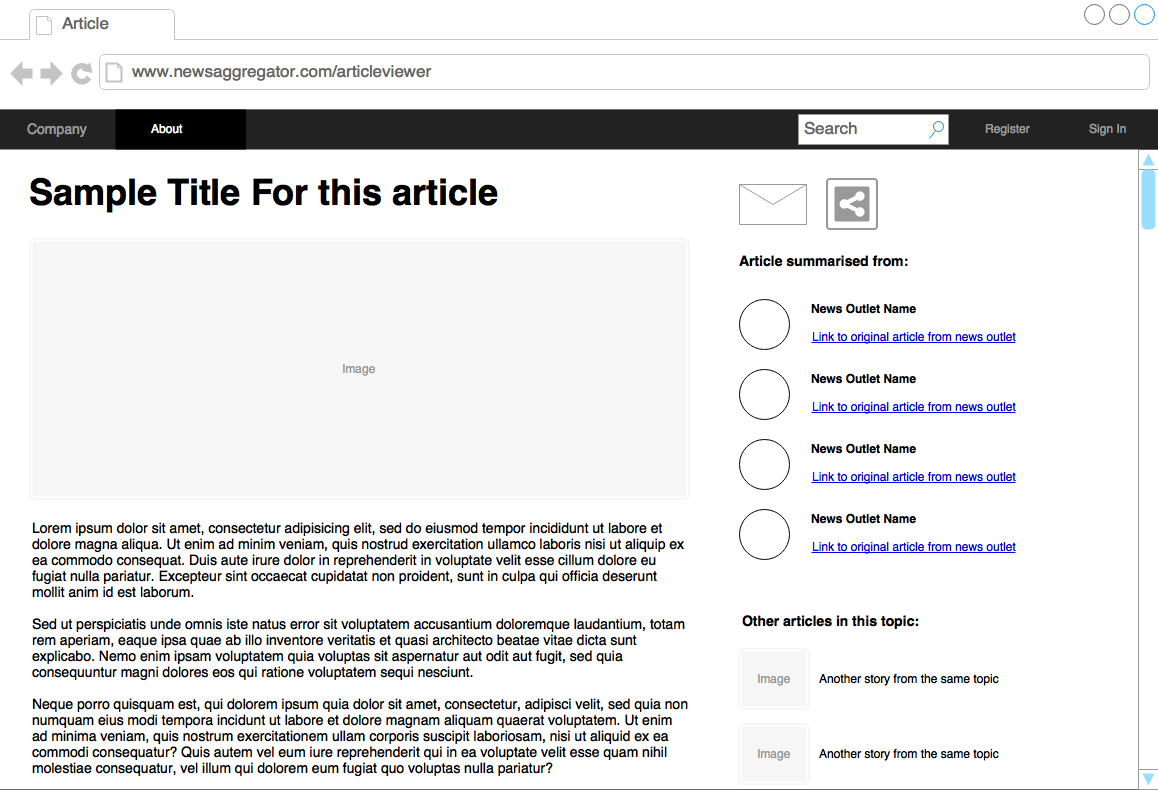
\includegraphics[scale=0.3]{ArticleViewer.png}
   \caption[A wireframe of the Article Viewer]{The Article Viewer is modelled on standard news outlets' interfaces.}
   \label{articleViewer}
\end{figure}

\subsubsection{Topic Lists}

The Topic List page is accessed by clicking on the profile button when logged in to the application. A panel appears, listing two choices - My Topics, and My Settings. This page is presented on the selection of the My Topics button.

The aim of the topic list is self-explanatory. It lists all topics that a user is subscribed to. Upon clicking on a topic in the list, a user would be taken to the Topic Settings page for that topic.

\begin{figure}[ht!]
  \centering
    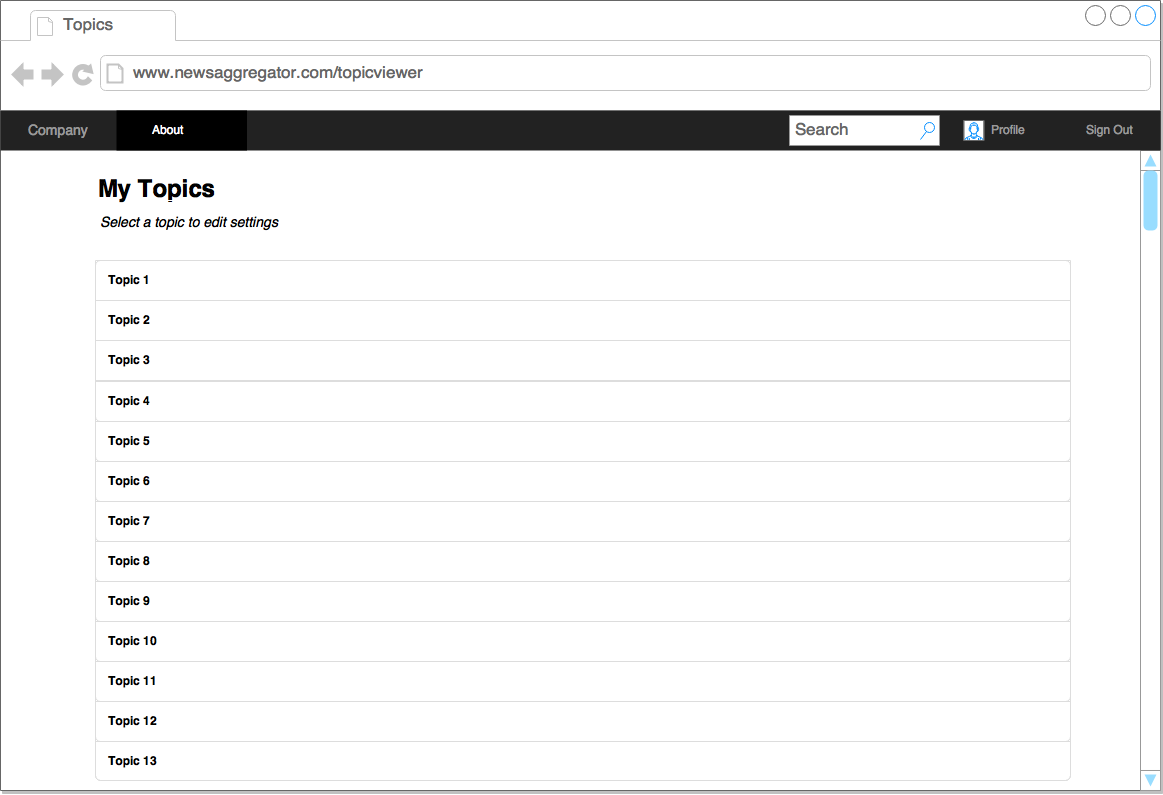
\includegraphics[scale=0.3]{UserTopics.png}
   \caption[A wireframe of the Topic List page]{The Topic List page allows users to select and adjust the settings of a topic.}
   \label{userTopics}
\end{figure} 

\subsubsection{Profile Settings}

The other option upon clicking on the profile button in the navigation bar of the application is to access the Profile Settings page. Here, the user is able to change their profile picture using the button in the top half of the page. Also present on this page are the user's digest settings. Here the user can set whether they want to receive a news digest in the morning, the afternoon, at both times, or not at all. They can also specify the email address that they wish the news digest to be sent to.

\begin{figure}[ht!]
  \centering
    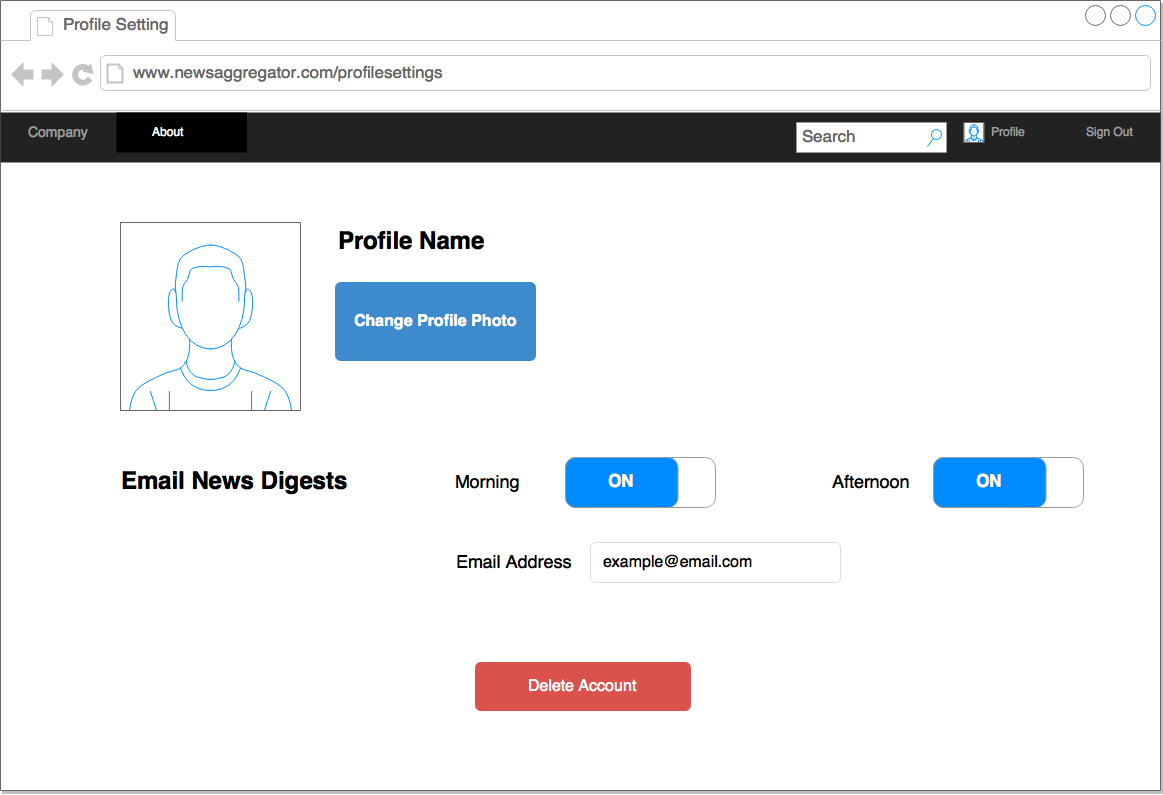
\includegraphics[scale=0.3]{ProfileSettings.png}
   \caption[A wireframe of the Profile Settings page]{The profile settings page allows the user to adjust their profile picture and digest settings.}
   \label{profileSettings}
\end{figure}

\subsection{Back End\index{Back End} Flow Diagram}

In Figure \ref{backEndArchitecture} the expected flow of the machine learning aspects of the back end is presented. The process of an article being summarised is as follows:

\begin{enumerate}
	\item The \textbf{Article Fetcher} queries the various News APIs used for new articles. \\
	\item The \textbf{Article Curator} takes the response from the News APIs and performs any scraping that may be necessary, before passing the article to the Machine Learning phases. \\
	\item The article is then passed to the \textbf{Topic Modelling}\textbf{Topic Modelling} phase, which identifies which topics it consists of. \\
	\item The \textbf{Topic Labelling}\index{Topic Labelling} section takes the results of the Topic Modelling phase, and proceeds to label its topic \\
	\item \textbf{Clustering}\index{Clustering} then occurs. The article, along with its topic label is passed to this phase, and the program pulls articles from the database that have already been assigned the same topic. These articles are then clustered, and the cluster containing this article is passed to the next phase. \\
	\item Now that the cluster has been passed, \textbf{Summarisation}\index{Summarisation} occurs on the article, which is then put in the Summarised Articles database, ready to be called for a user to read. \\
\end{enumerate}

\begin{figure}[ht!]
  \centering
    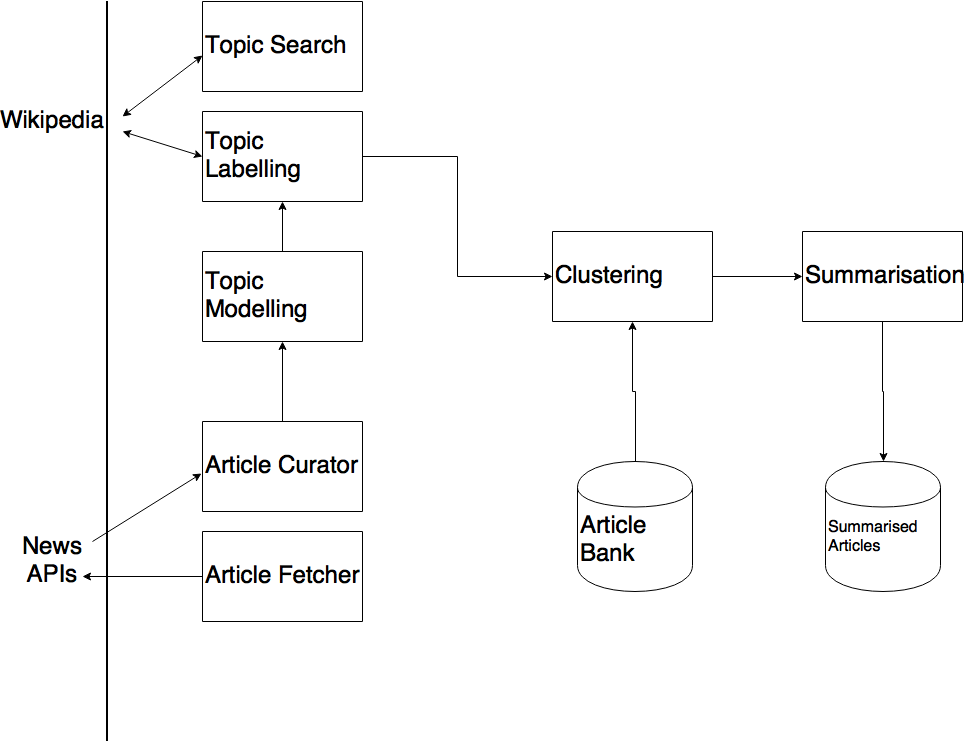
\includegraphics[scale=0.4]{BackEndArchitecture.png}
   \caption[A guide to the expected flow of the Back End]{The expected flow of the Back End.}
   \label{backEndArchitecture}
\end{figure}

\subsection{Language and Platform Choices}

\subsubsection{Front End}

The survey\index{Survey} that was conducted in Section \ref{survey} clearly presented the result that a website would be the preferred option for the application, followed by a mobile application in either iOS or Android. Therefore I've decided to follow this and create a WebApp as a primary platform. If time permits, I'll then develop the application for a second platform, which will be a mobile platform.

For the WebApp I will primarily use Bootstrap for the Interface. One design framework I used to great effect during my Industrial Placement in Summer 2016 was React and Redux\index{Redux}\index{React}. React is a JavaScript library developed by Facebook that is designed for building scalable and reusable user interfaces. Redux is a design pattern for JavaScript that is designed around a central predictable state container that is the single source of truth for a User Interface. 

The benefit of this framework is that it allows for very clean code in the user interface. This is because the concept of a single source of truth allows for data flow that is purely in only one direction, making it easier to understand.

\subsubsection{Back End}

The back end will be constructed using Java. The reasoning behind this is that I have experience from my Industrial Placement using Java as the basis of a server and a back end.

\newpage

\printbibliography[heading=bibintoc]
\newpage
\printindex


\end{document}